\RequirePackage[hyphens]{url}
\documentclass[american]{emisa}

% \usepackage{todonotes}

% \newcommand{\noteSM}[1]{\todo[color=red!40, author=\textbf{Salvador}, inline, caption={}]{#1}}
 \newcommand{\noteJC}[1]{\todo[color=pink!40, author=\textbf{JC}, inline, caption={}]{#1}}
% \newcommand{\noteSylvain}[1]{\todo[color=green!40, author=\textbf{Sylvain}, inline, caption={}]{#1}}
% \newcommand{\noteAntoine}[1]{\todo[color=yellow!40, author=\textbf{Antoine}, inline, caption={}]{#1}}
% \newcommand{\noteFabien}[1]{\todo[color=orange!40, author=\textbf{Fabien}, inline, caption={}]{#1}}
% \newcommand{\noteJoel}[1]{\todo[color=blue!20, author=\textbf{Joel}, inline, caption={}]{#1}}
 \newcommand{\noteFahad}[1]{\todo[color=purple!20, author=\textbf{Fahad}, inline, caption={}]{#1}}

\emisainitialism{\EMF}{EMF}
\emisainitialism{\MOF}{MOF}
\emisainitialism{\MDE}{MDE}
\emisainitialism{\FML}{FML}

\usepackage{bookmark}
\usepackage{multirow}
\usepackage{listings}
%\usepackage[hyphens]{url}
%\usepackage{xcolor}
%\usepackage{hyperref}
%\usepackage{tikz-uml}
%\usepackage{float}
%\usepackage{algorithmic,algorithm}

\newcommand{\mpc}{MULTI process challenge\xspace}%keep it for the moment
\newcommand{\mlpc}{Multi-Level Process Challenge\xspace}

\newcommand{\inst}[1]{\textsf{'#1'}}

\newcommand{\req}[2]{\textsf{#1}$_{#2}$}
\newcommand{\reqp}[1]{\req{P}{#1}}
\newcommand{\reqs}[1]{\req{S}{#1}}
%\newcommand{\reqp}[1]{\textsf{P}$_{#1}$}
%\newcommand{\reqs}[1]{\textsf{S}$_{#1}$}

\definecolor{codegreen}{rgb}{0,0.6,0}
\definecolor{codegray}{rgb}{0.5,0.5,0.5}
\definecolor{codepurple}{rgb}{0.58,0,0.82}
\definecolor{backcolour}{rgb}{0.95,0.95,0.92}
\definecolor{tableShade}{gray}{0.9}

%\DeclareTextFontCommand{\mytexttt}{\ttfamily\hyphenchar\font=45\relax}

\lstdefinelanguage{fml}{
  keywords={
    abstract,boolean,break,byte,case,catch,char,class,%
    const,continue,default,do,double,else,extends,false,final,%
    finally,float,for,goto,if,implements,import,instanceof,int,%
    interface,label,long,native,new,null,package,private,protected,%
    public,return,short,static,super,switch,this,throw,%
    throws,transient,true,try,use,void,values,volatile,while,with,String},%
  morekeywords={
    [3]concept,model,forEach,assert,%
  },%
  sensitive,%
  morecomment=[l]//,%
  morecomment=[s]{/*}{*/},%
  morestring=[b]",%
  morestring=[b]',%
}

\lstdefinestyle{mystyle}{
    backgroundcolor=\color{backcolour},
    commentstyle=\color{codegreen},
    keywordstyle=\color{magenta},
    numberstyle=\tiny\color{codegray},
    stringstyle=\color{codepurple},
    basicstyle=\ttfamily\scriptsize,
    breakatwhitespace=false,
    breaklines=true,
    flexiblecolumns=true,
    captionpos=b,
    emptylines=0,
    tabsize=2
}

\lstset{style=mystyle,language=fml}

\hypersetup{
  pdfauthor={Sylvain Guérin, Joel Champeau, Jean-Christophe Bach, Antoine
  Beugnard, Fabien Dagnat, Salvador Martinez},
  pdftitle={Multi-level modeling with Openflexo/\FML -- A contribution to the \mlpc},
  unicode=true,
  breaklinks=true,
  pdfkeywords={Multi-Level Modeling Challenge, Federation Modeling Language,
  Openflexo},
  %abstract
  pdfsubject={Model federation is a multi-model \emph{management} approach based on the use of virtual models and loosely coupled links. The models in a federation remain autonomous and represented in their original technological spaces whereas virtual models and links (which are not level bounded) serve as control components used to present different views to the users and maintain synchronization. In this paper we tackle the \emph{MULTI process modeling challenge}, which consists in providing a solution to the problem of specifying and enacting processes. Solutions must fulfill a number of requirements for a process representation defined at an abstract process-definition level and at various more concrete domain-specific levels, resulting in a multi-level hierarchy of related models. We present a solution based on model federation and discuss the advantages and limitations of using this approach for multi-level modeling. Concretely, we use virtual models and more precisely the Federation Modeling Language ({FML}) that serves to describe them as the main building block in order to solve the process modeling challenge whereas the federation feature is used as a means to provide editing tools for the resulting process language. Our solution fulfills all the challenge requirements and is fully implemented with the Openflexo framework.}
}

\begin{document}
\begin{article}{
    % \title{\mpc: the FML solution}
    \title{Multi-level modeling with Openflexo/\FML}
    \subtitle{A contribution to the \mlpc} % A contribution to the Multi-Level Process Challenge

    %% or include affiliations in footnotes:
    \author{Sylvain Guérin}%{firstname.lastname@ensta-bretagne.fr}
    \address{ENSTA Bretagne, Lab-STICC, UMR 6285, Brest, France}
    % \ead{firstname.lastname@ensta-bretagne.fr}

    \author{Joel Champeau}
    \address[a]{}

    \author*{Jean-Christophe Bach}{jc.bach@imt-atlantique.fr}
    \address{IMT Atlantique, Lab-STICC, UMR 6285, Brest, France}
    % \ead{firstname.lastname@imt-atlantique.fr}

    \author{Antoine Beugnard}
    \address[b]{}

    \author{Fabien Dagnat}
    \address[b]{}

    \author{Salvador Mart\'inez}
    \address[b]{}

    \abstract{Model federation is a multi model \emph{management} approach based on the use of virtual models and loosely coupled links. The models in a federation remain autonomous and represented in their original technological spaces whereas virtual models and links (which are not level bounded) serve as control components used to present different views to the users and  maintain synchronization. In this paper we tackle the \emph{MULTI process modeling challenge}, which consists in providing a solution to the problem of specifying and enacting processes. Solutions must fulfill a number of requirements for a process representation defined at an abstract process-definition level and at various more concrete domain-specific levels, resulting in a multi-level hierarchy of related models. We present a solution based on model federation and discuss the advantages and limitations of using this approach for multi-level modeling. Concretely, we use virtual models and more precisely the Flexo Modeling Language (\FML) that serves to describe them as the main building block in order to solve the process modeling challenge whereas the federation aspect is used as a means to provide editing tooling for the resulting process language. Our solution is fully implemented with the Openflexo framework. It fulfills all the challenge requirements.

\noteSylvain{Ce qui m'embête un peu avec cet abstract c'est qu'on met en avant la fédération de modèles alors que sur ce cas précis on en fait pas vraiment (sauf pour la partie outillage avec les éditeurs diagrammatiques). Concernant la fédération de modèle proprement dite, je crois qu'il faut qu'on montre qu'on a besoin d'une couche conceptuelle (qu'on relie à l'espace technique via les connecteurs techniques, les model slots et les rôles). C'est ce besoin qu'adresse le language \FML. On montre ici plutôt que le language \FML - utilisé comme language conceptuel - est assez intéressant, assez expressif pour capturer les exigences du challenge d'une part, et va jusqu'à permettre l'exécution des processus. Et cerise sur le gâteau: on peut construire un outillage graphique pour editer et exécuter ce use case.}
\noteSylvain{En revanche, on peut arguer que pouvoir au même niveau manipuler modèle et métamodèle nous simplifie grandement les choses pour adresser des problématiques multi-niveaux > un bout de la conclusion}.
%The models in a federation remain autonomous and represented in their original technological spaces %whereas virtual models and links serve as control components used to present different views to the %users and  maintain synchronization. 
}
    \keywords{Model federation \and Multi-Level Modeling \and System modeling languages \and Abstraction, modeling and modularity \and Reusability }
    %ACM
    % Software and its engineering/Software notations and tools/System description languages/System modeling languages
    % Software and its engineering/Software organization and properties/Software system structures/Abstraction, modeling and modularity
    % Software and its engineering/Software creation and management/Software development techniques/Reusability
    \bibliography{biblio.bib}
}

\section{Introduction}
\label{sec:introduction}
\pdfbookmark[section]{Introduction}{sec:introduction}
Model-driven engineering (\MDE) has traditionally adopted a strict hierarchical
two-level approach, where metamodels reside in a certain meta-level, and models
are created one meta-level below by using types from the metamodel. Notable
examples of this approach are the widespread Eclipse Modeling Framework
(\EMF)~\parencite{emf} and the Object Management Group Meta-Object Facility
(\MOF)~\parencite{omg2013mof}.

This strict approach shows its limitations when modeling complex domains
requiring more than one level of specialization, \eg to adapt the model to
application subdomains. Indeed, the two-level approach fails to acknowledge and
support: 1) the existence of different forms of classification and/or
instantiation (\eg ontological vs linguistics); and 2) the duality type-object
for model elements. Therefore, while it may still be used for the
aforementioned complex modeling tasks, the strict approach entails the
introduction of accidental complexity in both the modeling process and the
resulting modeling artifacts.

In order to tackle this problem, the \emph{multi-level} modeling paradigm has
been introduced. Contrary to the strict approach, multi-level modeling
advocates the use of a flexible number of levels as well as more flexible
relations between them. %{\color{red} The article of ICSE by me and Fabien can be
%cited here} {(JC) \color{pink} Effectivement. intégré dans la liste}
This paradigm is gaining traction within the modeling community as evidenced by
the contribution of many new multi-level modeling approaches and tools such as
Melanee~\parencite{melanee}, LIMM~\parencite{icse2011-limm},
MetaDepth~\parencite{metadepth}, MultEcore~\parencite{multecore2016},
DeepTelos~\parencite{deeptelos2016} or DMLA~\parencite{dmla2017}. Taking
advantage of this vibrant state of affairs, and in order to foster discussion
and enable comparison between competing approaches, a multi-level modeling
challenge has been created for the MULTI workshop. This paper is a response to
the latest multi-level modeling challenge~\parencite{multiProcessChallenge-emisaj}
%\footnote{It can be found here: \url{http://purl.org/emisajchallenge}. It is an updated version of the challenge used in~\textcite{multiProcessChallenge2019}}
which consists in providing a solution to the problem of specifying and
enacting processes. Solutions to the \emph{Multi-level Process Challenge} must
fulfill a number of requirements for a process representation defined at an
abstract process-definition level and at various more concrete domain-specific
levels, resulting in a multi-level hierarchy of related models. In this
article, we respond to this challenge using a solution based on model
federation~\parencite{Golra2016-federation}.

Model federation is a multi-model management approach based on the use of
virtual models and loosely coupled links. The models in a federation remain
autonomous and are represented in their original technological spaces whereas
virtual models (also called conceptual models) and links that serve as control
components used to present different views to the users and maintain
synchronization. Our solution is based on the model federation infrastructure.
Concretely, we use Openflexo and its internal Federation Modeling Language
(\FML), a language to create, link and manage virtual models, in order to solve
the MULTI process challenge while the federation feature is used solely so as
to provide tools for the resulting process language. Our solution, which is
fully implemented and executable, meets all the requirements.
%\noteFabien{Le paragraphe qui précède me semble redire des choses de la
%section 2, comment fait-on ?}

Our modeling approach is based on a language (\FML) which provides the
(linguistics) concepts that are used to define the multi-level models and
meta-models that are needed. \FML allows defining models as first class
entities (which we call \emph{virtual models}) and linking them together (by
extension). In the \mpc case study, we exploit this possibility to:
\begin{itemize}
    \item Define, extend and adapt models, keeping the history, to meet the %changing
    modeling requirements of the case study,
    \item Align this hierarchy of models with requirements evolution
      (\reqp{1}--\reqp{19} then \reqs{1}--\reqs{13}).
\end{itemize}
This methodological choice allows us to adapt the models and keep track of their evolution each time the requirements evolve.

Contrary to a classical multi-level approach, in which the notion of
multi-level is integrated in the language and must therefore be respected, our
approach allows building multiple levels on demand, and with the appropriate form.
Without multilevel-specific operators/concepts, the \enquote{custom}
construction must be done explicitly during the model development and evolution
process.

Our solution to the challenge is therefore not a response using a classical multi-level approach that would allow an efficiency comparison with another classical multi-level solutions, but an approach that proposes another organization of multi-level hierarchy through the translation of needs into levels over time and the possibility to build an evolving hierarchy of adapted models. This is made possible by (1) the reification of the notion of a model and (2) the possibility to interconnect models (specialization).% and (2) the freedom of meta-modeling (low model conformity, flexible meta-modeling).

%Links among models can be within a same level of abstraction or across levels of abstractions which gives,

%as our answer to the challenge shows, a great flexibility.

The rest of the paper is organized as follows. Sect.~\ref{sec:technology}
presents our approach and the technology it relies on. Sect.~\ref{sec:analysis}
is the analysis of the problem. We detail our model in Sect.~\ref{sec:model}
and show how it satisfies the challenge requirements in
Sect.~\ref{sec:requirements}. We assess the modeling solution in
Sect.~\ref{sec:discussion}. Sect.~\ref{sec:relatedwork} presents the related
work before the conclusions.%~\ref{sec:conclusions}.


% \cite{multiProcessChallenge2019}

% \emph{Submissions responding to the challenge should describe
% a multi-level model conforming to the case description,
% including justifications for non-trivial design decisions. In
% order to foster comparability between solutions, respondents
% are asked to make sure that concepts of the case description
% are explicitly represented by one or more model elements.}\\

% \emph{criteria:
% \begin{enumerate}
%     \item Does the response address the established domain as described in the challenge description and demonstrate the use of modeling features?
%     \item Does it evaluate/discuss its proposed modeling solution against the criteria described in the challenge description?
%     \item Does it discuss the merits and limitations of the employed modeling technique?
%     Authors are invited to suggest further requirements to demonstrate particular benefits of the approaches they adopt.
% \end{enumerate}
% }

% structure : plus ou moins imposée par le challenge (structure actuelle = sections au moins attendues)


%\noteSM{test}
%\noteJC{test}
%\noteSylvain{test}
%\noteAntoine{test}
%\noteFabien{test}
%\noteJoel{test}

\section{Technology}
\label{sec:technology}
\pdfbookmark[section]{Technology}{sec:technology}
%Technology: precise description of the technology / approach that is used

% Inspiré de la section 10 du papier formose

To meet the \mlpc, we have decided to use the general
approach of model federation~\parencite{Golra2016-federation}. \emph{Model
  federation} is a way to assemble models using some kind of
low-coupling links. It has been studied to answer the \OMG' RFP
Semantic Modeling for Information Federation~\parencite{simf}. In
contrast to approaches that compose metamodels into a single large
metamodel grouping all needed entities, model federation build links
between models and metamodels (even through levels) to make ``things''
work together. As an illustration of this feature, we developed a
free-modeling editor -- freeing oneself from the bonds of
model/metamodel conformity -- that is presented
in~\parencite{models2016-freemodel}. Another notable feature of
this approach is the strong decoupling among tools that remain usable
after federations are made.

We decided to use this approach since it offers the possibility to
link and to navigate among levels. Before we describe the overall
architecture in next section, here are some key concepts implemented
in the Openflexo~\parencite{openflexo_link} framework.

% figure
% Dans la suite les références à la figure sont commentés

\begin{figure}[t]
    \centering
    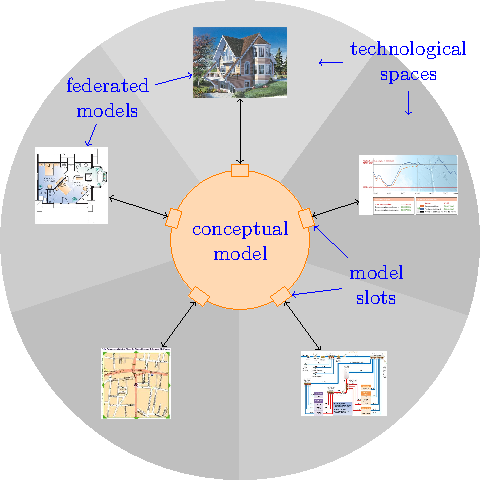
\includegraphics[width=\columnwidth]{Figures/federation.pdf}
    \caption{The model federation approach}
    \label{fig:mf}
\end{figure}

This framework relies on the architecture of Figure~\ref{fig:mf}. A federation
gathers a set of conceptual models, named \emph{virtual models} and a
set of \emph{federated models}. Each federated model pertains to a
\emph{technological space} and uses the language of its specific
paradigm while a virtual model is built using the Flexo Modeling
Language (\FML). Each federated model is an autonomous
element that may evolve with its own tooling. The virtual models
serve as control elements binding the federated models together.
In this paper, we mainly use conceptual models and more precisely \FML its domain specific modeling language. The only use of the federation aspect is on the tooling made for the process language.

\begin{figure}[t]
    \centering
    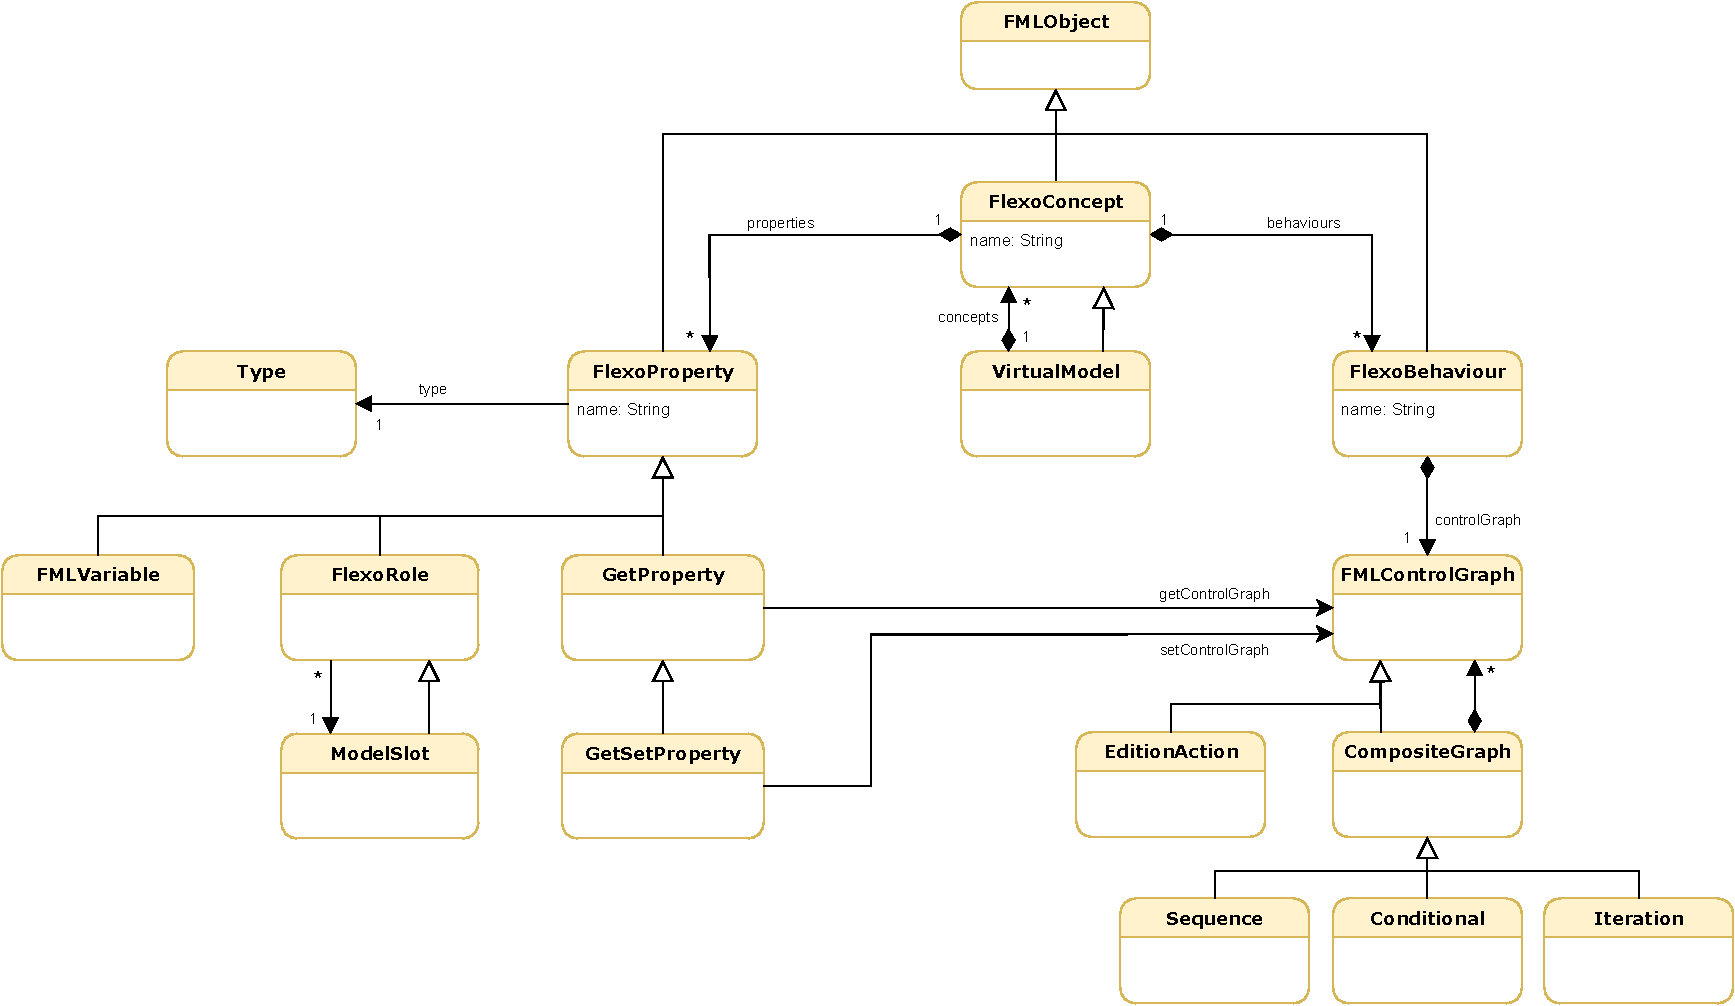
\includegraphics[width=\columnwidth]{Figures/FMLMetaModel.pdf}
    \caption{Internal representation of \FML language}
    \label{fig:mm}
\end{figure}
%\noteAntoine{Dans la figure ne manque-t-il pas les containements ? (VM vers Concepts)}

\FML simplified metamodel is provided in Figure~\ref{fig:mm}. It is designed to define models as virtual models. A virtual model
is composed of a set of \emph{concepts}, while itself being a concept.
Hence, virtual models are structuring units forming architectures while concepts are the
core entities. A concept has a set of \emph{roles} and
\emph{behaviors}. A parallel to object-oriented approach can be useful
to understand \FML\footnote{Some aspects of \FML do not exist in object oriented approach.}. A concept corresponds to a class, its roles to the
attributes of the class and its behaviors to the methods of the class.
These roles have types defining the kind of value the role will point
at runtime.
Whenever a type external to the federation space is used, one needs to use a \emph{model slot}. A model
slot is a mediation entity in charge of giving
access to external elements using
a \emph{technology adapter}\footnote{It is a reusable library that defines
connections between the \FML execution engine and a particular
technological space.}.

\FML is designed to define not only the structure of virtual models but
also to define the collection of actions an engineer can perform on
them. These actions are called \emph{behaviors} and can either be called (like usual methods) or triggered by events. The reactive behaviors are mainly useful when a federated model evolution needs to trigger a computation. We do not
exploit this possibility in the challenge.


When the \FML execution engine runs a federation, it creates virtual
model instances containing concept instances. Some concept instances
are connected to external elements through model slot instances.


The tool support for model federation framework,
Openflexo\footnote{\url{https://github.com/openflexo-team}}, is
developed as an open source initiative. This tool offers a \FML
execution engine with an interactive virtual model design environment.

Finally, tools have their own model. We have taken advantage of
Openflexo features to build, in parallel with the models  required by the challenge, a drawing tool that makes our
solution (partially) executable.


\section{Analysis}
\label{sec:analysis}
\pdfbookmark[section]{Analysis}{sec:analysis}
%\emph{Analysis: any disambiguations of the  case  description and assumptions made, any potentially added requirements}

During the requirement analysis of the challenge, the foundation of our reflections and modeling intentions is guided by the general model federation approach. 

In a first step, the federation approach is mainly based on modeling relationships between several models, independently of their abstraction level and the model architecture.

During the next step of our approach, we try to take into account the reusability of the relationships by identifying the semantics of each relationship. The goal is the identification of concepts with their behavior. The last step is to organize or structure these concepts to improve reusability and extensibility, to create virtual models in \FML terminology.     

Like in a lot of modeling approaches, these  steps could also be achieved in any order and iteratively. But our goal during the challenge's analysis remains to produce a \FML virtual model architecture for our federation. 
As shown in figure~\ref{fig:MultilevelArchitecture}, we defined two virtual models (Base and Acme processes abstractions) instantiated by two virtual model instances (XSure and Acme processes). As the figure shows the virtual models play the role of metamodels, in the sense of concept definition with a level-agnostic approach. The virtual model instances play the role of models conforming to the metamodel definitions. In the rest of the paper, we use the term metamodel and model to simplify the presentation.
The resulting architecture follows the way the challenge is presented and this
organisation allows for the possibility of flexible extensions.


\begin{figure}[t]
    \centering
    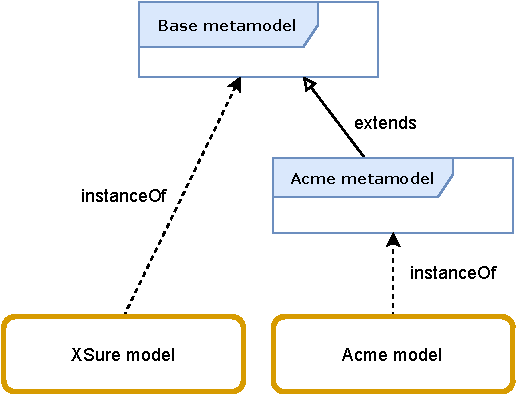
\includegraphics[width=0.7 \columnwidth]{Figures/MultilevelArchitecture.pdf}
    \caption{Multilevel architecture of our solution}
    \label{fig:MultilevelArchitecture}
\end{figure}

Our analysis of the use case leads to identify two main modeling axis (as presented in figure \ref{fig:LinguisticAndOntologicInstantiation}):
\begin{itemize}
    \item The horizontal axis is characterized as the ontological instantiation axis, in the sense that the domain type definition (\ie \texttt{ProcessType}) is referenced by an instance definition (\ie \texttt{Process}). In our base metamodel, each domain type definition is referenced by its instance definition, as developed in the section \ref{sec:ProcessEnactment}

\item The vertical axis is viewed as the linguistic instantiation, relative to the use of the \FML language. The virtual model, defined as the core definition metamodel, generates a model founded on the instantiation mechanism of the \FML Language. This mechanism is similar to the classical object/instance mechanism of the object languages but without any constraint on the referenced virtual model, \ie metamodel. The set of resulting instances comes from several virtual models 
of any abstraction level as detailed in section \ref{sec:AcmeSoftwareDevelopmentProcess}


\end{itemize}

\begin{figure}
    \centering
    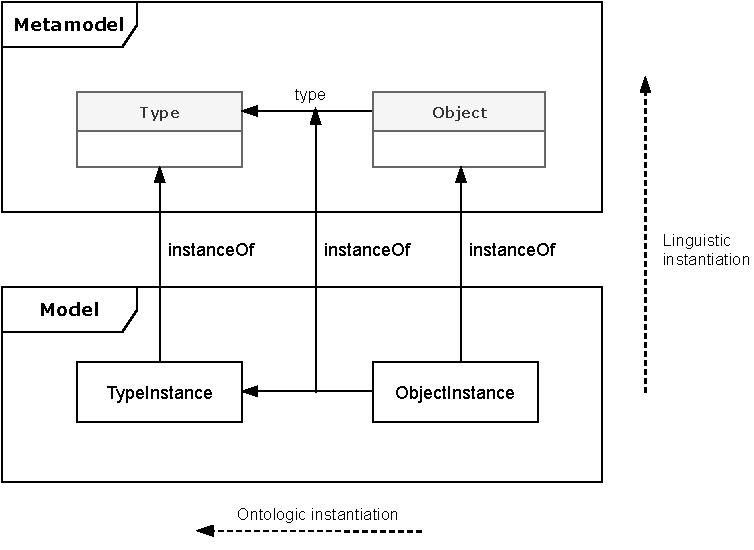
\includegraphics[width=1.0 \columnwidth]{Figures/Instantiation.pdf}
    \caption{Linguistic and ontologic instantiation}
    \label{fig:LinguisticAndOntologicInstantiation}
\end{figure}

Based on this approach, we organize our set of models following the architecture of the aforementioned Figure \ref{fig:MultilevelArchitecture}. The resulting multi-level architecture is organized in two virtual models, one for the core concepts metamodel containing the definition of Processes and Tasks, and one, the Acme metamodel, extending the previous model to integrate the Acme definitions. The \FML language defines multiple inheritance concept between virtual models as illustrated in the section~\ref{sec:AcmeSoftwareDevelopmentProcess}.

Finally as explained previously, the defined level for the Acme  and the XSure models is the result of the instantiation of virtual models. In our approach this virtual model instance level can't be specialized or extended but all the other virtual models could be extended by any concepts, as a new federated model. 
Also, the instance level can be instantiated from any virtual model, which represent any metamodel level. 

\noteAntoine{Pourquoi S9 et S13 sont ambigus, quels choix on a fait...}
\todo[inline]{noms pas dans la spec, complètement implicite ; }

We now analyse a few specifications that deserve a comment for the choices we made. 

\begin{itemize}
    \item We added an implicit specification (S0) saying that all things have names.
    \item (S9) It is unclear when a tested artefact must be associated to its test report. At the creation of the artefact or of its report? \todo[inline]{We choose\dots}
    \item (S13) [linked to P9] \todo[inline]{We choose ti interpret \dots}
\end{itemize} 

% cross level constraints or added models as federated metamodels


%\todo[inline]{quelles hypothèses supplémentaires ?}
%\todo[inline]{+ architecture de la modélisation (ce qui se trouve dans le ppt), le détail se retrouvera dans la section suivante}


\section{Model presentation}
\label{sec:model}
\pdfbookmark[section]{Model presentation}{sec:model}
%Model Presentation: detailed  presentation of a model, including justifications for design decisions

The presentation of our solution to the \mpc follows a systematic methodology where modeling choices are introduced step by step, as the requirements are stated. Satisfaction of requirements is explained throughout this presentation.

%\todo[inline]{phrase d'intro pour expliquer que les req étaient couverts au fur et à mesure (côté systématique)}

The designed multilevel architecture shown in Figure~\ref{fig:MultilevelArchitecture} captures the two use cases described in the Process Challenge.

% Expliquer que le use case XSure ne nécessitait pas l'extension de metamodèle requise pour le usecase Acme Software Developement Process

\subsection{Base metamodel for the Process Challenge}

\begin{figure*}
 \centering
    % 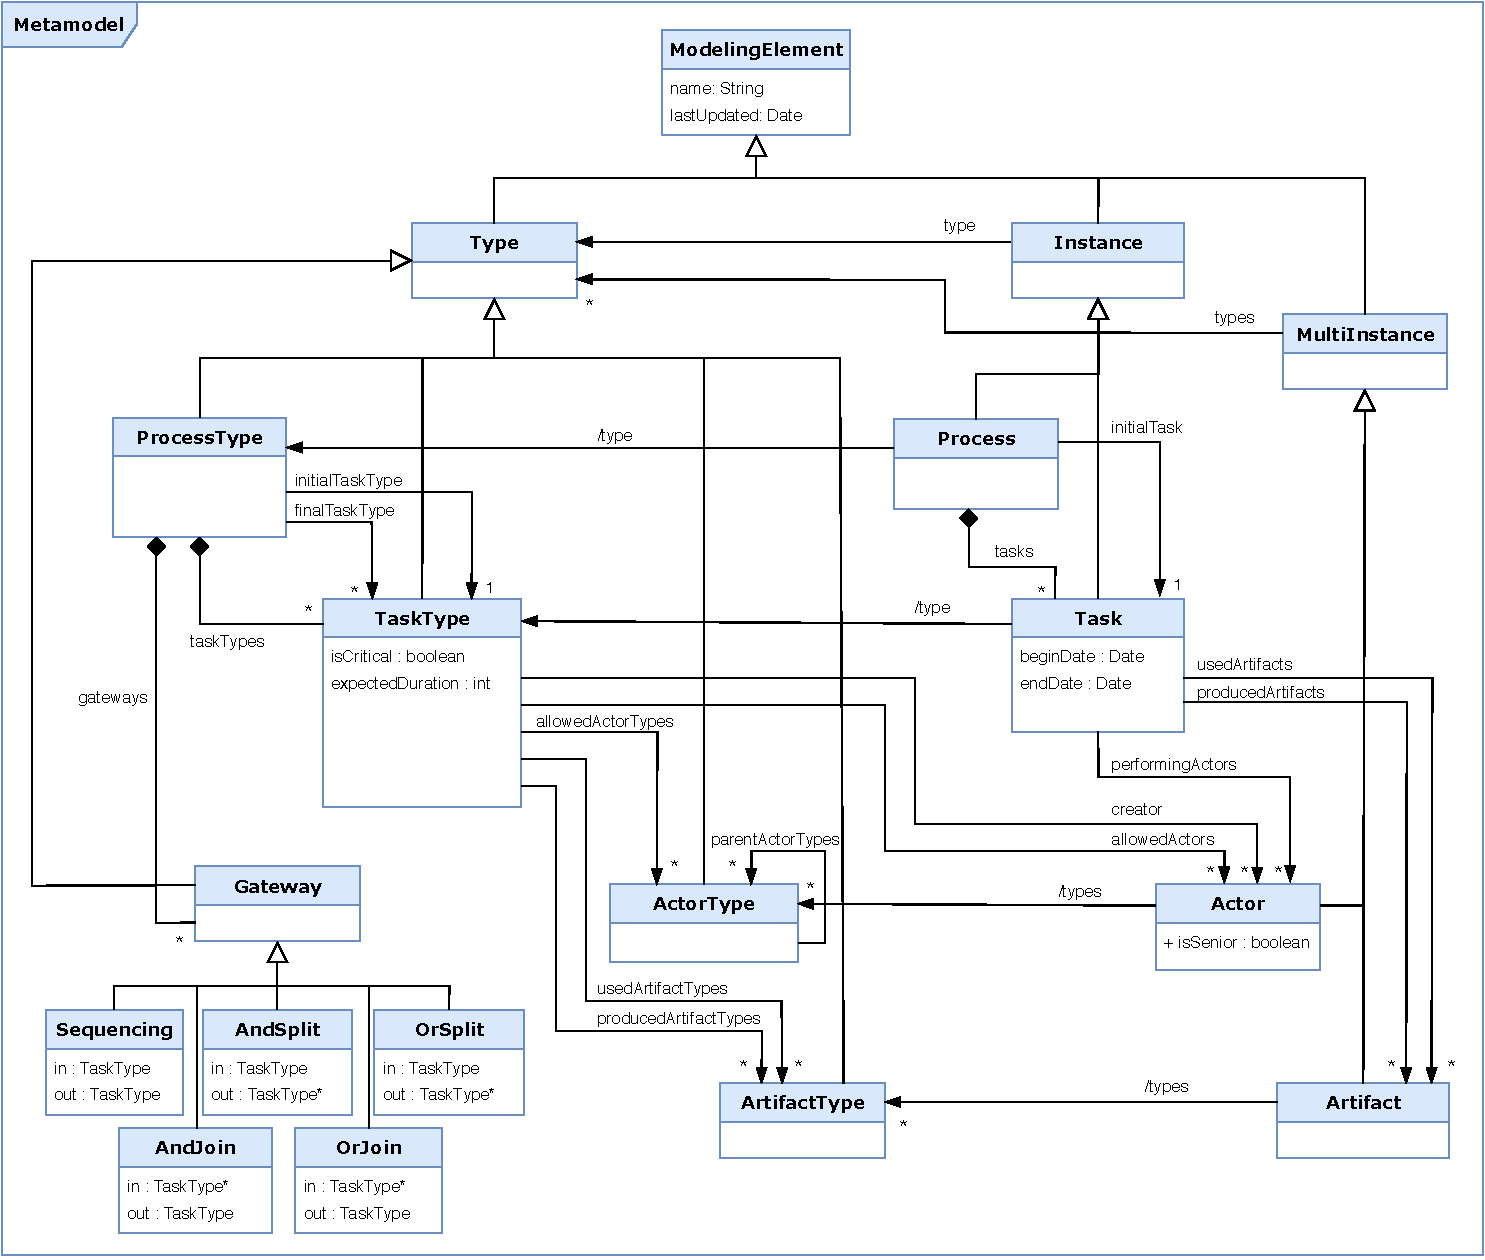
\includegraphics[width=1.0 \columnwidth]{Figures/Metamodel.pdf}
    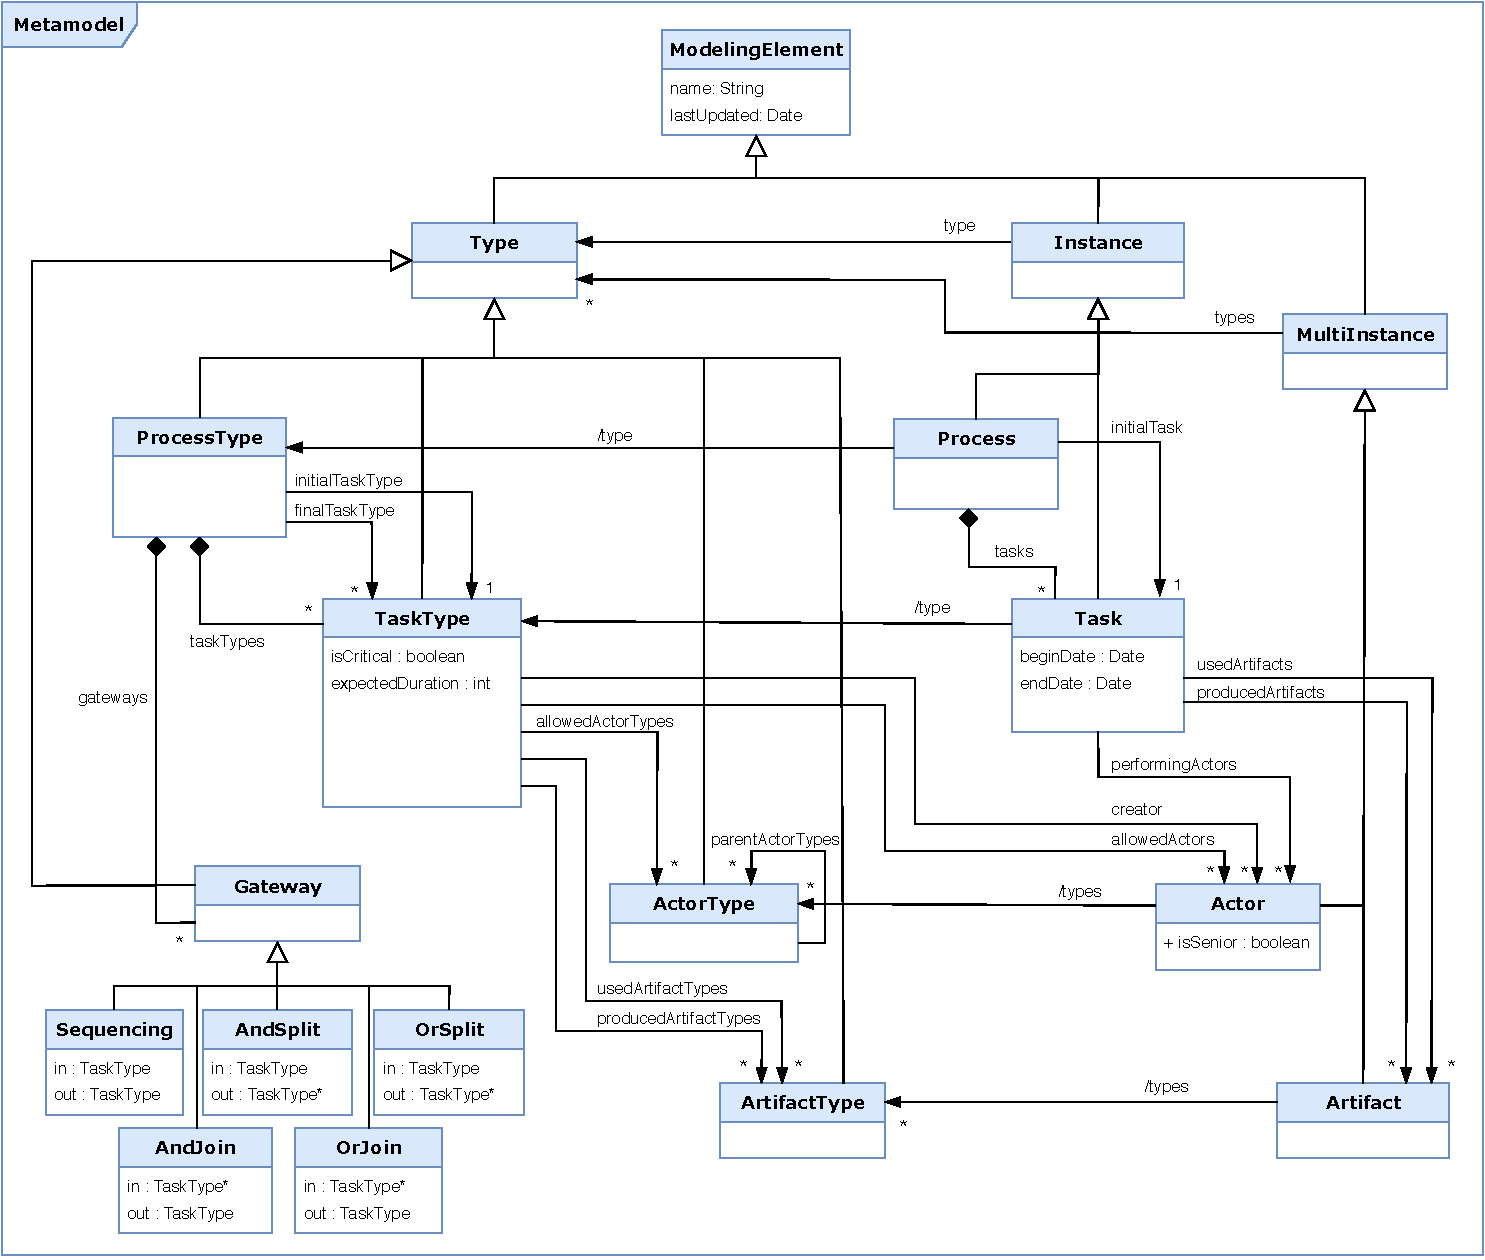
\includegraphics[width=1.0 \textwidth]{Figures/Metamodel.pdf}
     \caption{Process management base metamodel}
    \label{fig:BaseMetamodel}
\end{figure*}

In this section, we present the base metamodel presented in figure~\ref{fig:BaseMetamodel} with \textit{XSure} insurance domain use case, whose partial description was provided in the challenge description. The requirements \textbf{P1} to \textbf{P19} of XSure insurance domain are straightforwardly implemented by instantiating the \emph{XSure model}, as an instance of base metamodel (the left side of figure~\ref{fig:MultilevelArchitecture}).

Figure~\ref{fig:BaseMetamodel} represents this base metamodel with a \UML-like formalism, well adapted to represent \FML concepts and their instances. A \textit{Concept} of \FML is represented by a \UML class where roles of basic types are attributes. The roles whose types are concepts are represented by a combination of a name in their containing concept and an arrow from their name to their type. The cardinality follow the \UML practice.
For example, the role \texttt{parentActorTypes} of the concept \texttt{ActorType} has the type \texttt{ActorType} and the * cardinality.

Our proposition relies on ontologic instantiation as presented in figure \ref{fig:LinguisticAndOntologicInstantiation}, with a common root concept \texttt{ModelingElement}. Two types of ontological instantiation are needed to meet the requirements of the challenge. One provides that some instances conform to only one type (\texttt{Process} and \texttt{Task} do respectively conform to \texttt{ProcessType} and \texttt{TaskType}). While some entities define their conformity to several types (\texttt{Actor} and \texttt{Artifact} do respectively conform to several \texttt{ActorType} and \texttt{ArtifactType}). These instantiations are respectively expressed using the relations \texttt{type} and \texttt{types} between \texttt{Type}, \texttt{Instance} and \texttt{MultiInstance} concepts. In the diagram, the realization of these relations are indicated by a derived relation, \texttt{/type} or \texttt{/types}, as for example between \texttt{Process} and \texttt{ProcessType} or between \texttt{Actor} and \texttt{ActorType}.

\subsubsection{Process type definition}

We first present the process definition part of base metamodel, located left of figure \ref{fig:BaseMetamodel}.

% Illustrer avec des instances de XSure

\texttt{ProcessType} is a specialization of the \texttt{Type} concept, and references a collection of \texttt{TaskType} through the composition relation \texttt{taskTypes} with (0..*) cardinality (\textbf{P1}). A \texttt{TaskType} is embedded in a \texttt{ProcessType} and inherits from its context. To illustrate this in \textit{XSure} insurance domain use case, \textit{XSure model} defines \textsf{Claim Handling}, instance of \texttt{ProcessType}, and \textsf{Receive Claim}, \textsf{Assess Claim} and \textsf{Pay premium}, instances of \texttt{TaskType}.

\texttt{ProcessType} also references a collection of gateways, reified with the \texttt{Gateway} concept hierarchy. \texttt{Gateway} is a specialization of \texttt{Type} and is specialized by \texttt{Sequencing}, \texttt{AndSplit}, \texttt{AndJoin}, \texttt{OrSplit} and \texttt{OrJoin} concepts (\textbf{P2}). Depending on its type and following its underlying operational semantics, a gateway defines one or more inputs and one or more outputs. A \texttt{ProcessType} additionally exposes a unique initial \texttt{TaskType} and a collection of final \texttt{TaskType} with both roles \texttt{initialTaskType} (single cardinality) and \texttt{finalTaskType} (cardinality 0..*) (\textbf{P3}). \texttt{TaskType} exposes a creator role as a reference to an \texttt{Actor} concept (\textbf{P4}), which is at the same conceptual level. 

The following listing shows an excerpt of the \FML code modeling some core concepts of process modeling base metamodel. 

\begin{lstlisting}
model MetaModel {

  concept ModelingElement { ... }
  
  concept Type extends ModelingElement { ... }
  
  concept ProcessType extends Type {
    TaskType[0..*] taskTypes;
    TaskType initialTaskType;
    TaskType[0..*] finalTaskTypes;
    Gateway[0..*] gateways;
        
    concept TaskType extends Type {
      Actor creator;
      Actor[0..*] allowedActors;
      ActorType[0..*] allowedActorTypes;
      ...
    }
        
    abstract concept Gateway extends Type {
      abstract void execute(Process process);
      ...
    }
        
    concept Sequencing extends Gateway {
      TaskType in;
      TaskType out;
    }
    
    // Other core concepts
  }
}    
\end{lstlisting}


The \texttt{ActorType} concept is a sub-concept of \texttt{Type} and the \texttt{allowedActorTypes} relation to \texttt{ActorType} defined in \texttt{TaskType} (with 0..* cardinality) captures \textbf{P5} requirement. Requirement \textbf{P6} is symmetrically satisfied with \texttt{allowedActors} relation to \texttt{Actor} also defined in \texttt{TaskType} (with 0..* cardinality). The same modeling pattern applies to \texttt{ArtefactType} defined as a sub-concept of \texttt{Type}, and both relations \texttt{usedArtifactTypes} and \texttt{producedArtifactTypes} defined in \texttt{TaskType} (\textbf{P7}). \texttt{TaskType} additionally exposes an \texttt{expectedDuration} role (expressed in number of days), satisfying \textbf{P8}.
\noteFabien{expectedDuration pas dans la figure}

The \texttt{Actor} concept defines a boolean attribute called \texttt{isSenior}, while \texttt{TaskType} defines an additional \texttt{isCritical} boolean attribute, indicating that some instance are flagged as critical and must be performed by senior actors. To fulfil \textbf{P9} requirement, a supplementary constraint is required for \texttt{TaskType} and is captured through the following invariant expressed in the \FML language:

\begin{lstlisting}
forEach (actor : allowedActors) {
    assert !isCritical | actor.isSenior
}
\end{lstlisting}

This invariant should be completed with additional constraints defined in the \texttt{Task} concept, which apply to performing actors assigned to enact tasks. 

\todo{Gérer également la fin de P9, non traité pour le moment: artifact they produced must be associated with a validation task}

\subsubsection{Process enactment}
\label{sec:ProcessEnactment}
We now present the process enactment part of base metamodel, located right of figure~\ref{fig:BaseMetamodel}. All concepts defined in this subsection are either specialization of the \texttt{Instance} concept (if they have exactly one type) or the \texttt{MultiInstance} concept (when they have several types).

\texttt{Process} represents an enacted \texttt{ProcessType}, as defined in previous subsection (\textbf{P10}). FML defines behavioral features called behavior. \texttt{ProcessType} defines the behavior \texttt{newProcess(String)}, taking the name of the process to enact as argument:

\begin{lstlisting}
public Process newProcess(String name) {    
  Process newProcess = new Process(name,this);  
  for (taskType : taskTypes) {      
    Task newTask = taskType.newTask(newProcess.name+"-"+taskType.name),newProcess);        
  }      
  return newProcess;    
}    
\end{lstlisting}

This scheme rely on \FML dynamic binding mechanism to delegate to task types the responsibility of instances creation. An instance of \texttt{Process} references its unique type \texttt{ProcessType} by the specialized \texttt{/type} role. Each instance of \texttt{TaskType} is ontologically instantiated with a \texttt{Task} (\textbf{P11}), using the same pattern where \texttt{TaskType} has the responsibility to manage the ontological instantiation. A \texttt{Task} references its unique \texttt{TaskType}, and defines a \texttt{begin date} and an \texttt{end date} basic role (\textbf{P12}).
\noteFabien{endDate en double}

The same pattern applies for the used and produced artifacts by roles \texttt{usedArtifacts}, \texttt{producedArtifacts} and \texttt{performingActors} defined in \texttt{Task} (\textbf{P13}). An instance of \texttt{Artifact} specializes \textit{MultiInstance} and references a set of \texttt{ArtifactType} through the specialized \texttt{/types} role (\textbf{P14} and \textbf{P16}). Likewise, \texttt{Actor} specializes \texttt{MultiInstance} and references a set of \texttt{ActorType} through the specialized \texttt{/types} relation (\textbf{P15}).

The semantics is unclear relatively to the instantiation policy for artifacts. We assume that task execution implies that for each used and produced \emph{artifact type} defined in a related \emph{task type}, it exists at least one \emph{artifact} declaring required ontologic instantiation (through \textit{type} role). The following excerpt of \FML code shows a partial implementation of this. The same pattern applies to produced artifacts.
\noteFabien{Je ne suis pas bien sûr de comprendre le paragraphe}

\begin{lstlisting}
concept Task extends Instance {
  ...
  boolean declaresRequiredUsedArtifacts() {
    for (artifactType : type.usedArtifactType) {
      boolean found = false;
      for (artifact : usedArtifacts) {
        if (artifact.isOfType(artifactType))
          found = true;
      }
      if (!found) return false;
    }
    return true;
  }
  ...
}    
\end{lstlisting}

Authorization for an actor to perform a task (\textbf{P17}) is captured either by the role \texttt{allowedActors} or the role \texttt{allowedActorTypes} defined in \texttt{TaskType}. This mechanism is completed by the behaviors \texttt{isAuthorizedActor}, \texttt{isValidActor} and \texttt{isValidActorType} defined in \texttt{TaskType}: 

\begin{lstlisting}
concept TaskType extends Type {
 ...
 // Check that an Actor is authorized to perform a task, using allowed Actor and ActorTypes
  boolean isAuthorizedActor(Actor actor) {      
    for (actType : allowedActorTypes) {        
      if (actor.hasActorType(actType))         
        return this.isValidActorType(actType);          
    }        
    for (act : allowedActors) {        
      if (actor == act)         
        return this.isValidActor(actor);
    }
    return false;
  }
  
 // Check that an Actor may perform this TaskType (override when required)
  boolean isValidActor(Actor actor) {
    return true;
  }

 // Check that an ActorType may perform this TaskType (override when required)
  boolean isValidActorType(ActorType actorType) {
    return true;
  }
  ...
}
\end{lstlisting}

The \texttt{Task} concept delegates this authorization to its task type, as shown in the following \FML code:

\begin{lstlisting}
concept Task extends Instance {
  ...
  boolean isAuthorizedActor(Actor actor) {      
    return type.isAuthorizedActor(actor);      
  }
  ...
}
\end{lstlisting}

Enforcing those constraints is finally performed by the definition of this invariant in the \texttt{Task} concept:

\begin{lstlisting}
forEach (actor : performingActors) {
  assert isAuthorizedActor(actor);
}
\end{lstlisting}

The default behavior states that all actors and actor types are valid for all task types. This modeling scheme offers many extension points, by the redefinition of some behaviors in the inherited concepts (although none were required in the context of \emph{XSure} use case).

Actor types specialization is captured by the \texttt{parentActorTypes} relation defined in \texttt{ActorType} (\textbf{P18}). This is completed by both the definition of the \texttt{hasActorType(ActorType)} behavior in \texttt{Actor} and the recursive behavior \texttt{isOrSpecializes(ActorType)} in \texttt{ActorType}:

\begin{lstlisting}
concept ActorType extends Type {
  ActorType[0..*] parentActorTypes;
  ...
  boolean isOrSpecializes(ActorType actorType) {    
    if (actorType == this)   
      return true;      
    for (p : parentActorTypes) {      
      if (p.isOrSpecializes(actorType)
        return true;
    }
    return false;
  }
  ...
}

concept Actor extends MultiInstance {
  ...
  boolean hasActorType(ActorType actType) {      
    for (type : types) {
      if (type.isOrSpecializes(actType))
        return true;
    }
    return false;
  }     
  ...
}
\end{lstlisting}

All concepts inherits from \texttt{ModelingElement}, which defines a \texttt{lastUpdated} attribute with \texttt{Date} type, and thus satisfies \textbf{P19} requirement. 

\subsection{The Acme software development process}
\label{sec:AcmeSoftwareDevelopmentProcess}

The challenge describes in a second part a Software engineering process for a fictional Acme company. Base metamodel as described in previous section is too generic to capture all domain-specific aspects of this use case. We choose to complete the architectual hierarchy with a specific VirtualModel, specific to Acme software development process metamodel, as shown in figure \ref{fig:AcmeArchitecture}. \textit{Acme} metamodel inherits and specializes base metamodel, and \textit{Acme model} is defined as an instance of \textit{Acme} metamodel. The metamodel inheritance is implemented as VirtualModel's inheritance. Any instance of Acme model is either an instance of a concept defined in base metamodel, or a concept defined in specialized Acme metamodel, which may or not inherit from a concept defined in base metamodel.
% FML follows a classical object-oriented semantics. ???

\begin{figure}
 \centering
    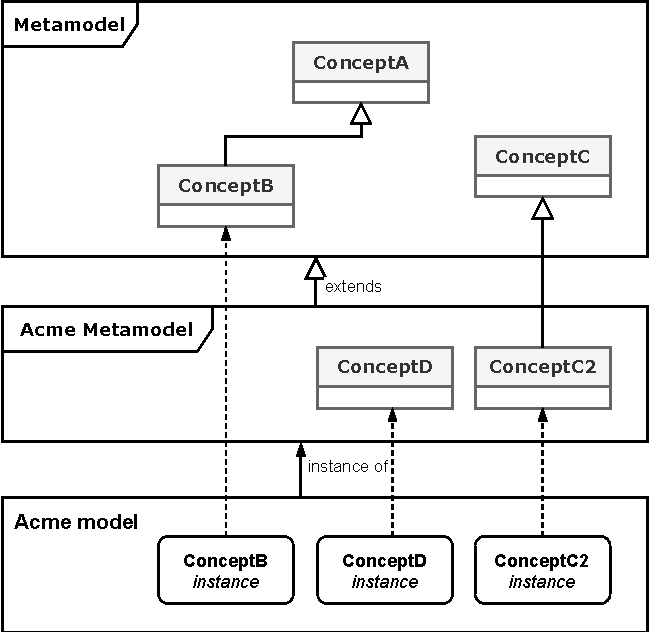
\includegraphics[width=1.0 \columnwidth]{Figures/AcmeArchitecture.pdf}
     \caption{Acme software development process architecture}
    \label{fig:AcmeArchitecture}
\end{figure}

\begin{figure*}
 \centering
     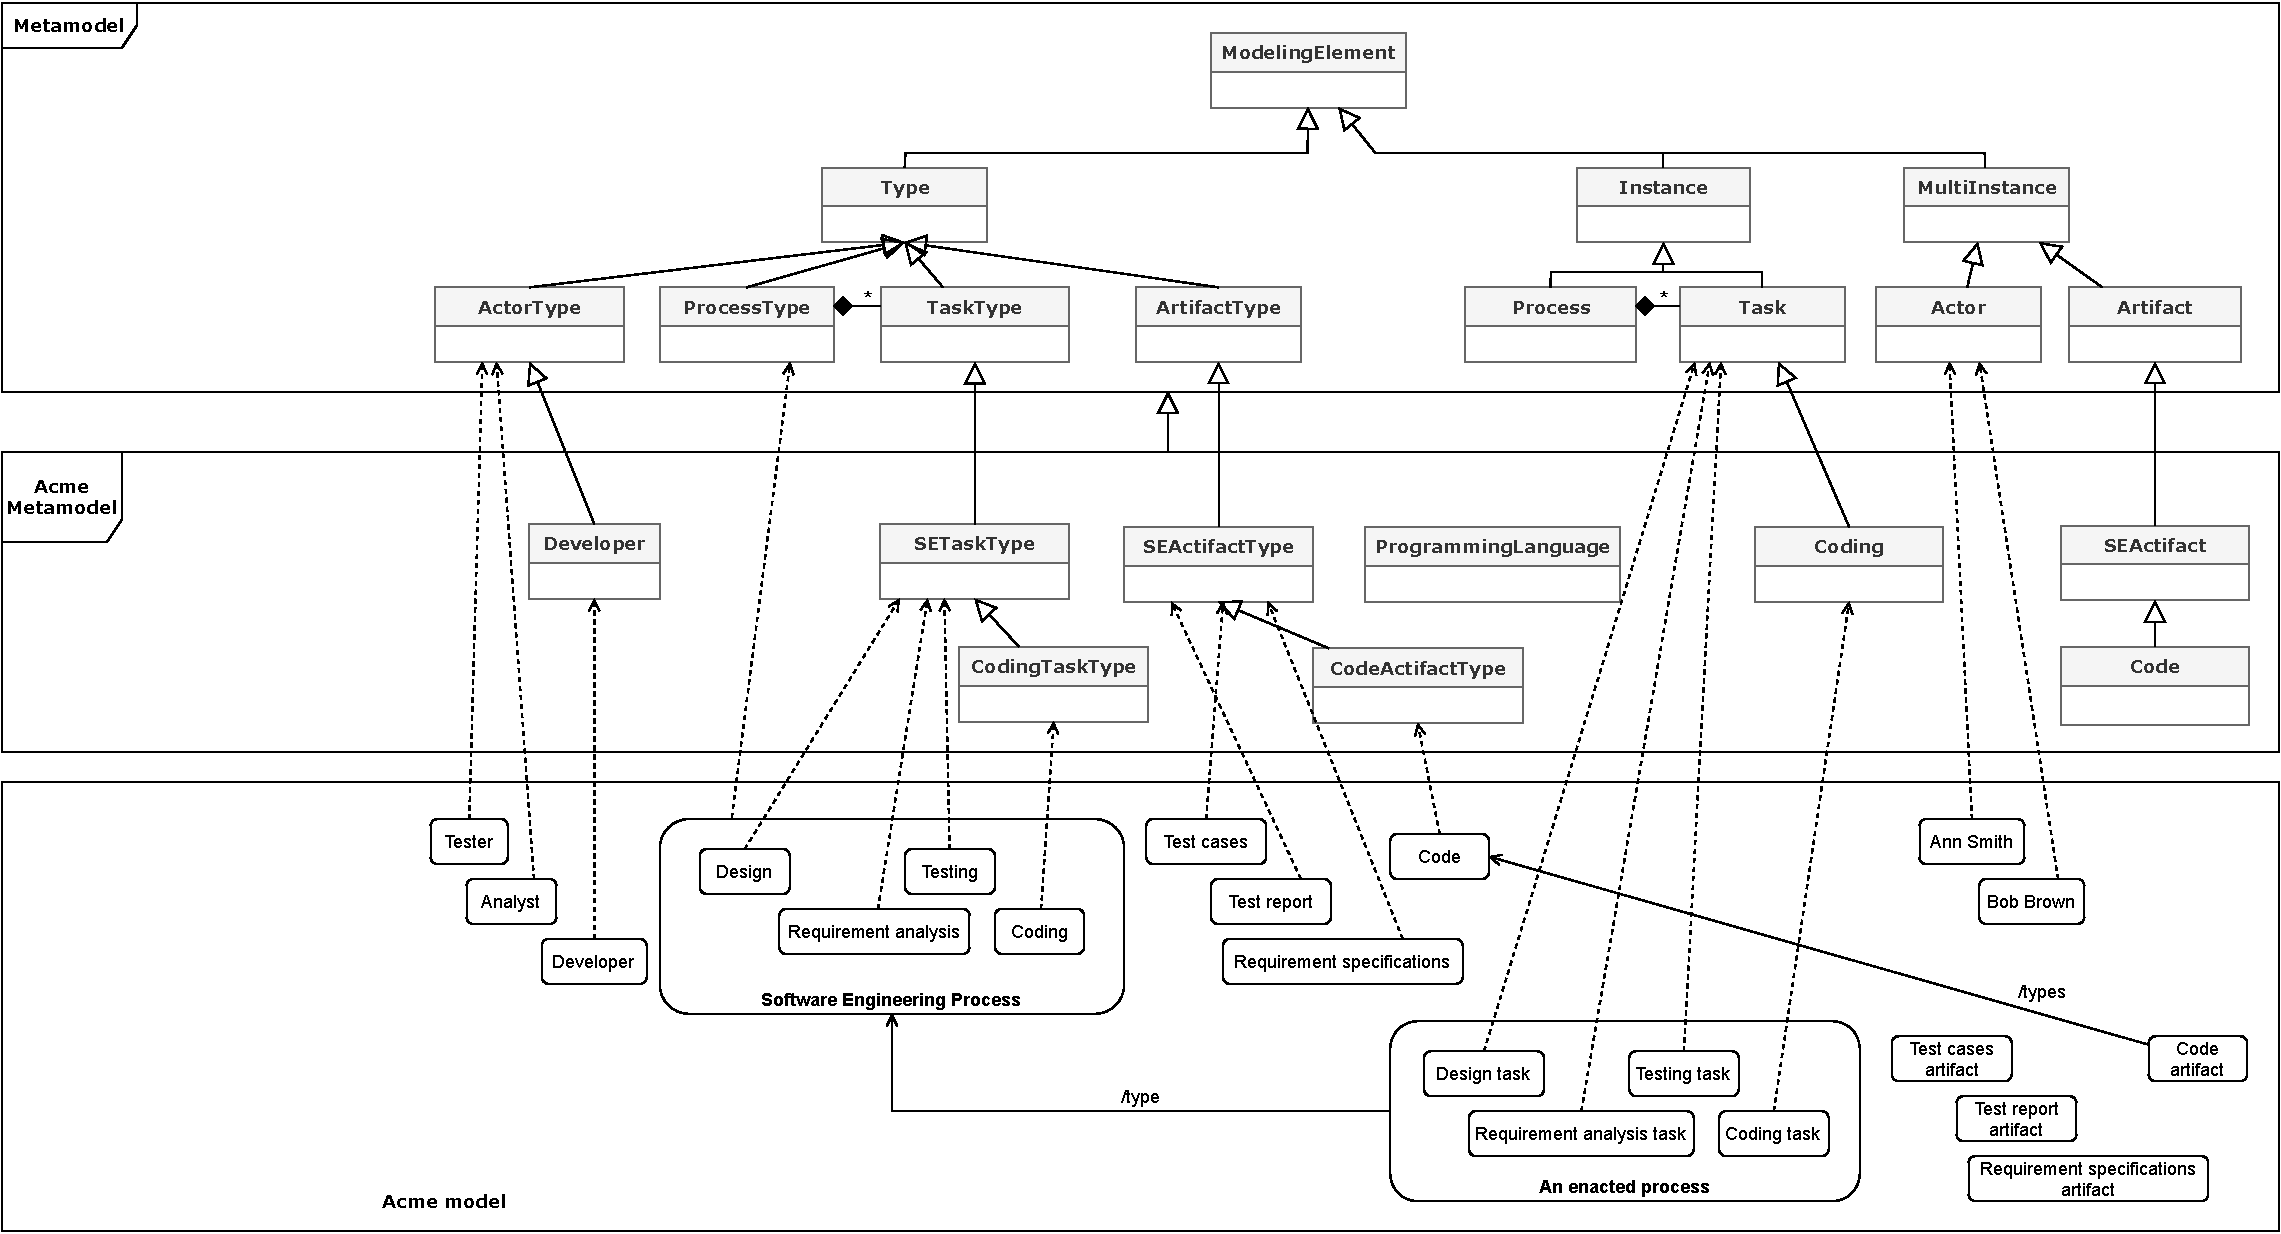
\includegraphics[width=1.0 \textwidth]{Figures/AcmeFullArchitecture.pdf}
     \caption{Acme software development process architecture}
    \label{fig:AcmeFullArchitecture}
\end{figure*}

\todo[inline]{Augmenter la taille des fontes de la figure \ref{fig:AcmeFullArchitecture}}
\todo[inline]{Ajouter les programming languages}

Figure \ref{fig:AcmeFullArchitecture} shows the full architecture capturing Acme software development process, with an instance of enacted \textit{Software Engineering Process}, and highlights all conceptual levels. Acme metamodel enriches base metamodel by offering specializing concepts: \textit{SETaskType} extending \textit{TaskType}, a more specialized concept \textit{CodingTaskType} extending \textit{SETaskType}, \textit{SEArtifactType} extending \textit{ArtifactType}, a more specialized concept \textit{CodeArtifactType} extending \textit{SEArtifactType}. Acme metamodel also defines task type \textit{Coding} as a specialized concept of \textit{Task}, and provides concept \textit{Developer} extending \textit{ActorType}. This metamodel is completed with \textit{ProgrammingLanguage} concept, defined as an enumeration (\textit{Java}, \textit{C}, \textit{COBOL}). All instances required to capture challenge use case are still defined in final Acme model itself instance of Acme metamodel. Instances are represented with rounded boxes and linguistic instantiation are represented with dashed connectors.

The \textit{Software Development Process} for Acme company is presented in the figure \ref{fig:AcmeSoftwareDevelopmentProcess} which is a screen-capture from the tooling developed in the context of the challenge and described in the next section. 

\begin{figure}
 \centering
    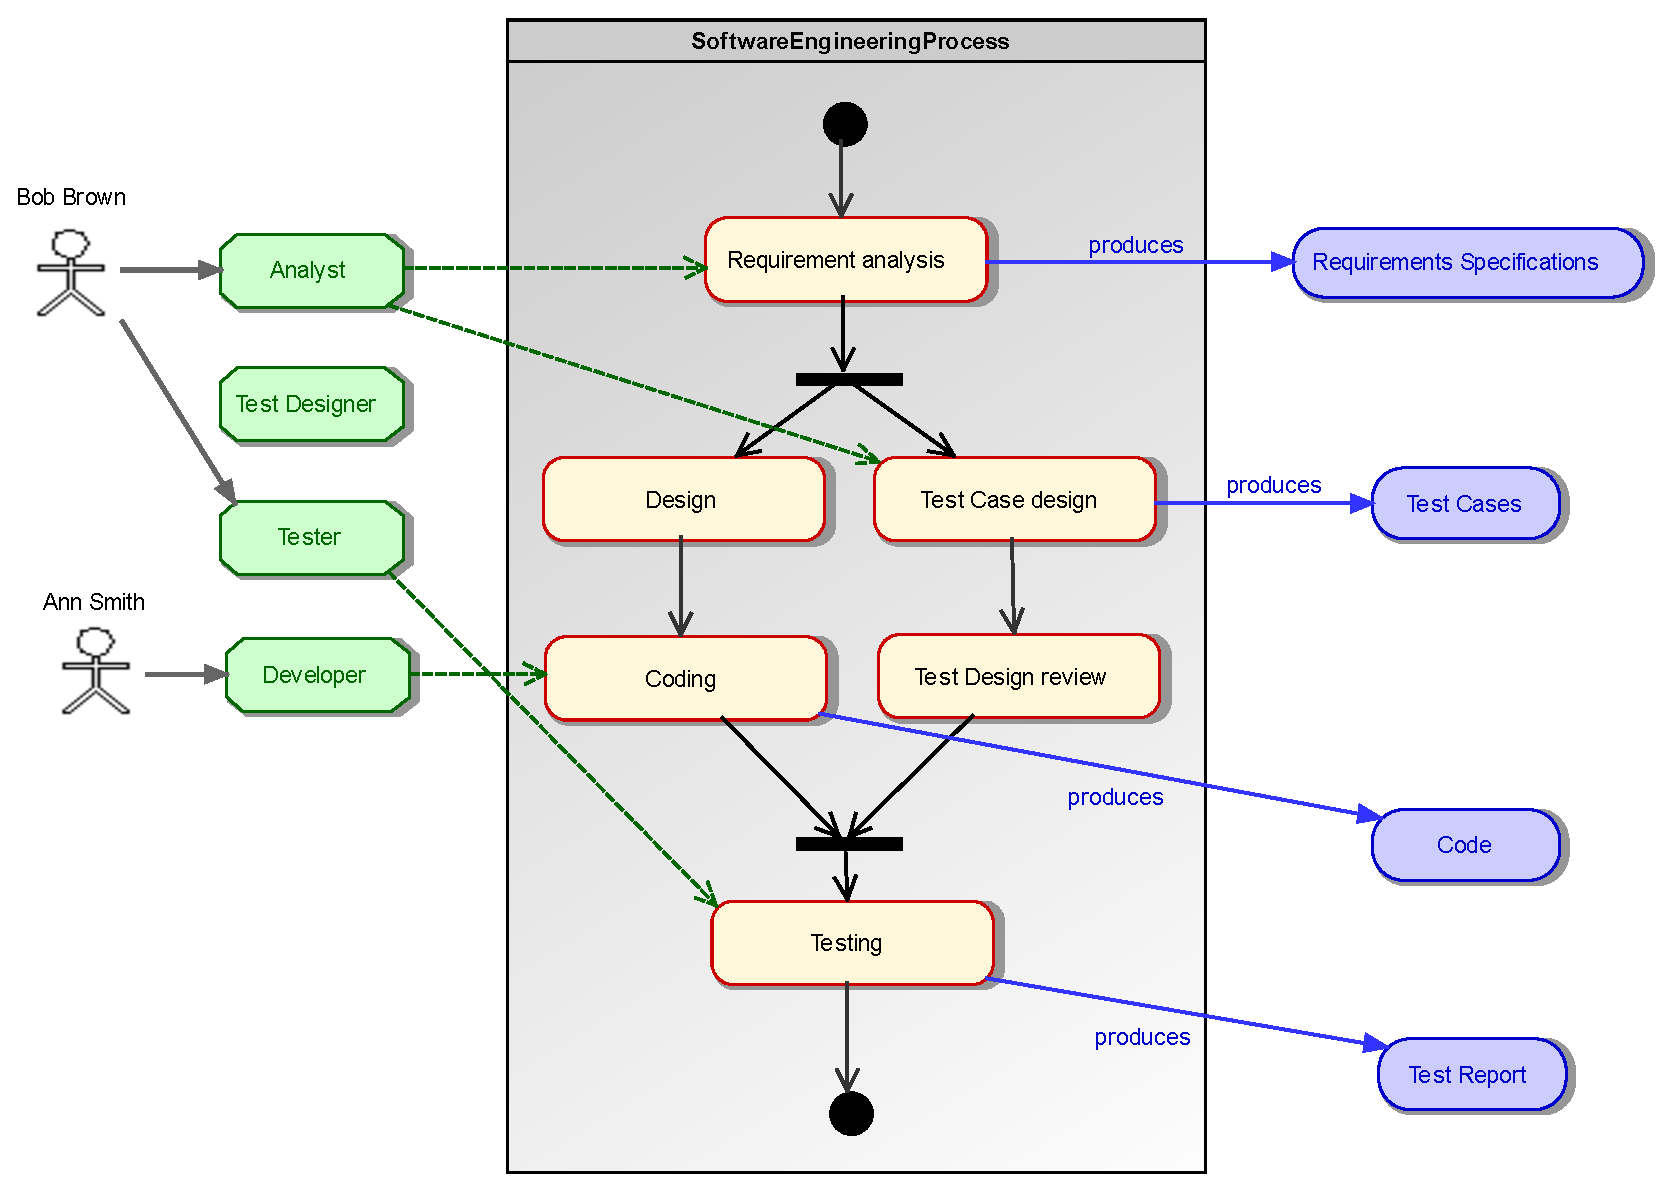
\includegraphics[width=1.0 \columnwidth]{Figures/SoftwareEngineeringProcessCroped.pdf}
     \caption{Acme software development process}
    \label{fig:AcmeSoftwareDevelopmentProcess}
\end{figure}

\textit{"Requirements analysis"} is defined as an instance of \textit{SETaskType}, \textit{Analyst} as an instance of \textit{ActorType} and \textit{Requirement specifications} as an instance of \textit{SEArtifactType}. \textit{"Requirements analysis"} instance defines property values \textit{producedArtifactTypes=\{Requirement specifications\}} and \textit{allowedActorTypes=\{Analyst\}} (\textbf{S1}). In the same way, \textit{"Test case design"} is defined as an instance of \textit{SETaskType}, marked as critical with property value \textit{isCritical=\{true\}}, and bound to \textit{Analyst} with \textit{allowedActorTypes} relation. \textit{"Test case design"} produces \textit{"Test cases"} defined as an instance of \textit{SETaskType}. The latter is used in "Test design review" (\textit{producedArtifactTypes} relation) (\textbf{S1} and \textbf{S13}, satisfied with \textbf{P9}). 

The capture of \textbf{S3} requirement is performed while defining \textit{Coding} as an instance of concept \textit{CodingTaskType} extending \textit{SETaskType} and defining a relation \textit{languages} to \textit{ProgrammingLanguage} with 1..* cardinality. \textit{newTask(String)} behavior overrides generic implementation while instantiating a \textit{Coding} concept, specializing \textit{SEArtifact}, as shown in following excerpt of FML code:

\begin{lstlisting}
concept CodingTaskType extends SETaskType {
  ProgrammingLanguage[1..*] languages;
  ...
  public Coding newTask(String name) { 
    return new Coding(name,this); 
  }
}    
\end{lstlisting}

\textit{Code} concept extends \textit{SEArtifact}, and defines a relation \textit{language} to \textit{ProgrammingLanguage} with single cardinality (\textbf{S4}). \textbf{S5} is more ambigous as task type \textit{Coding} defines one or more programming languages but produces code which is expressed in one language only. This requirement is captured through the redefinition of \textit{declaresRequiredProducedArtifacts()} where programming language should also match. 
\textbf{S6} is guaranteed though the \textit{language} relation defined in \textit{Code} and following invariant declared in \textit{Code}:  

\begin{lstlisting}
forEach (artifactType : types) {
  assert !(artifactType instanceof CodeArtifactType) | artifactType.doesImplement(languages)
}
\end{lstlisting}

\textit{Ann Smith} is the only one allowed to perform coding in COBOL (\textbf{S7}). This is implemented through the redefinition of \textit{newTask(String)} in \textit{CodingTaskType}:

\begin{lstlisting}
concept CodingTaskType extends SETaskType {
  ...
  public Coding newTask(String name) {
    Coding returned = new Coding(name,this); 
    if (languages.contains(ProgrammingLanguage.COBOL))
      returned.addToPerformingActors(getActor("Ann Smith"));
    return returned;
  }
}    
\end{lstlisting}

\textbf{S8} requirement is simply captured with the definition of \textit{Testing} instance of \textit{SETaskType}, \textit{Tester} instance of \textit{ActorType}, and \textit{Test report} instance of \textit{ArtifactType}.

\todo[inline]{requirement S9 non couvert pour le moment: compléter}


All software engineering artifacts defined in the context of Acme Software Engineering Process (figure \ref{fig:AcmeSoftwareDevelopmentProcess}) are all instances of \textit{SEArtifact} which defines both attributes \textit{responsible} (an \textit{Actor} instance), and \textit{versionNumber} (an \textit{integer} value), and thus fulfills \textbf{S10}. \textit{Bob Brown} is declared as an instance of \textit{Actor}, and references \textit{Analyst} and \textit{Tester} (\textit{ActorType} instances). He is also referenced by all instances of \textit{SETaskType} as the creator for related task types (\textbf{S11}).

\textbf{S12} is somehow ambiguous as it implies an implicit semantics regarding underlying business logic of process execution. We assume that all tasks may define an expected duration, which might be checked during process execution. This can be modeled through the addition of \textit{expectedDuration} attribute in \textit{TaskType}. Alternatively, this can be modeled through the definition of \textit{SETesting} concept, as a specialization of \textit{SETaskType}, and the instantiation of \textit{Testing} as an instance of \textit{SETesting}. The business logic expressed by \textbf{S12} requirement should be redefined in \textit{SETesting}.

\textbf{S13} requirement has been previously partially fulfilled. This must be completed with...

\todo[inline]{requirement S13 pas complètement couvert : compléter}

\subsection{Openflexo tooling}
\label{subsec:tooling}

Our solution is fully implemented within Openflexo tool. Both usecases have been modeled in the interactive design environment and are executable by the FML execution engine.

Base metamodel has been completed with some behaviors implementing execution semantic for executed processes. All tasks - instantiated from \textit{TaskType} for a given enacted process - manage a status which can be \textit{Not startable} (when not assigned to a performing actor or when required input artifacts are not available) , \textit{Startable}, \textit{Started}, \textit{Completable} (when all output artifacts are ready), \textit{Completed}). A \textit{Task} also manages a set of performing actors, a begin and end date, some used and produced artifacts. \textit{Gateways} business logic has also been implemented through the implementation of abstract \texttt{execute(Process)} behavior. Management of artifacts whose semantics follows rules defined in section \ref{sec:ProcessEnactment} (\textbf{P13}) has also been implemented.

We took advantage of model federation and the availability of diagramming features though the \textit{Diagramming TA} to implement two interactive graphical tools built on top of conceptual levels detailed in previous section. A first tool offers a graphical edition of a Process type, while the second tool offers enactment feature (the instantiation of a process from its process type), the ability within an enacted process to assign tasks to some actors, and the execution of this process with a graphical visualization.

\begin{figure*}
 \centering
     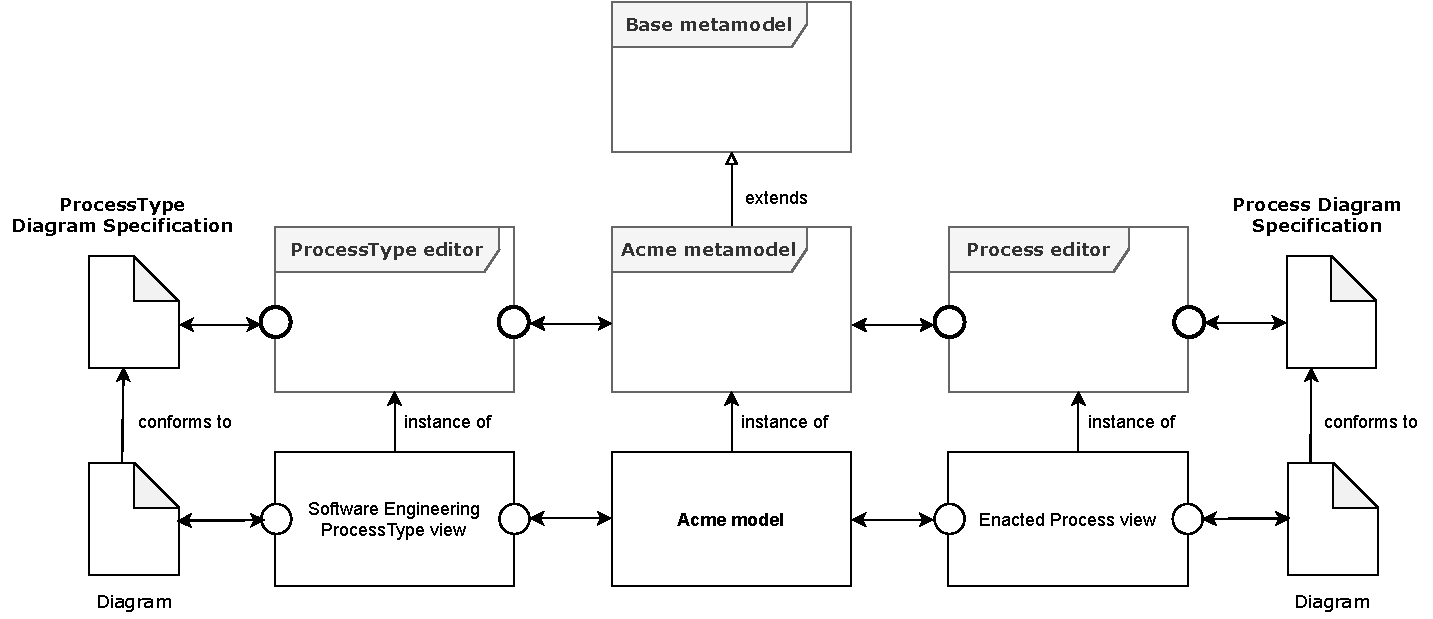
\includegraphics[width=0.9 \textwidth]{Figures/ToolingArchitecture.pdf}
     \caption{Tooling architecture}
    \label{fig:ToolingArchitecture}
\end{figure*}

Figure \ref{fig:ToolingArchitecture} shows the architecture of these two tools. Left of figure presents \textit{ProcessType graphical editor}. \textit{ProcessTypeEditor} is modeled as a \textit{VirtualModel} declaring two model slots (represented with bold circles). The first model slot references an instance of Acme metamodel, while the second model slot references an instance of diagram, conforms to the \textit{ProcessType diagram specification} (a diagram "metamodel" which defines and specify structure and graphical representations for edited items). While executed, this tool manages a graphical view for an instance of Acme metamodel (the \textit{Acme model}) and a specific \textit{ProcessType} instance. This tools allows to represent and edit a \textit{ProcessType}. One particular point should be noted regarding the highly reflective nature of FML and associated tooling : when drag and drop interactor is applied for a new item, the tool allows to choose the concept type to be instantiated (when a \textit{TaskType} is created for example, the user must choose the sub-concept of \textit{TaskType} to be selected - in Acme use case it can be \textit{SETaskTask} or \textit{CodingTaskType} or default value \textit{TaskType}). 

The other tool, called \textit{Enacted process graphical editor} and shown on figure \ref{fig:ScreenshotEnactedProcessEditor}, provides process edition and tasks assignations through a graphical visualization displaying process being executed. This tool is represented on the right side of the figure \ref{fig:ToolingArchitecture}. It follows the same architecture pattern as explicited for the \textit{ProcessType graphical editor}, with two model slots referencing both the model and a diagram. Process enactment is operated from a \textit{ProcessType}, and must be defined using a name identifying the newly instantiated process. All tasks are created from their \textit{TaskType} definition, and required assignments applies (if for example "Coding" \textit{TaskType} defines COBOL as output programming language, related task is automatically assigned to "Ann Smith"). All tasks get a status as well as a set of performing actors, a begin and end date, and used and produced artifacts. 

\begin{figure*}
 \centering
     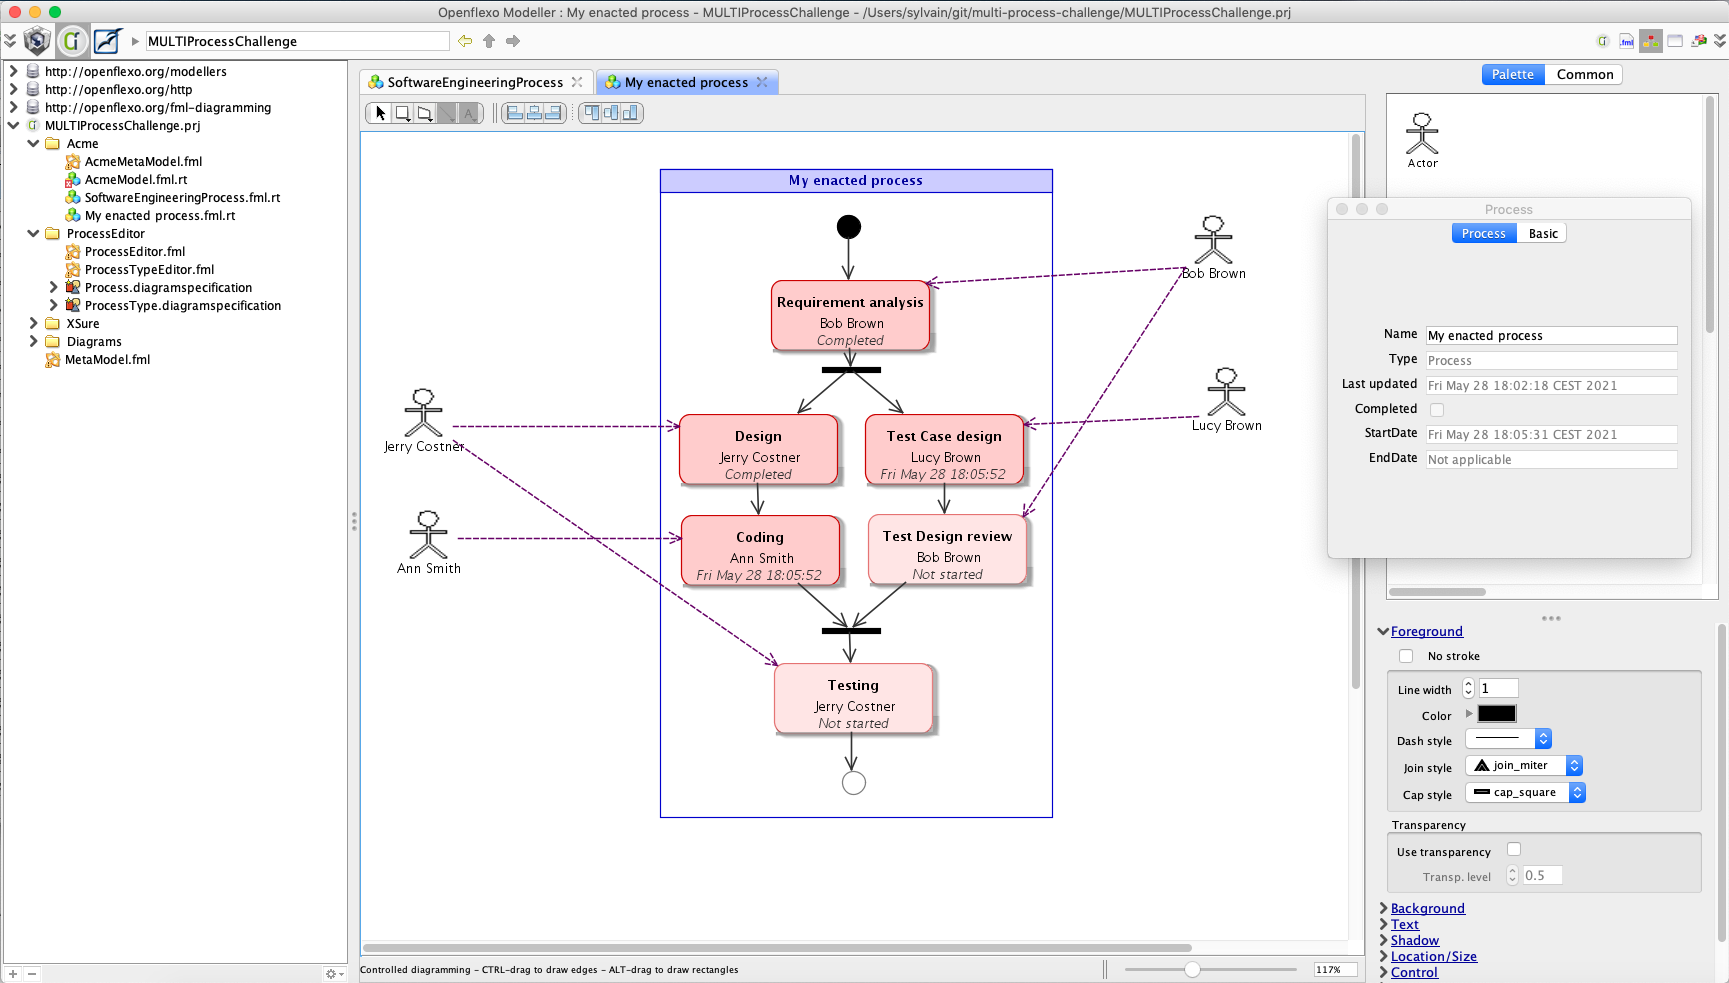
\includegraphics[width=1.0 \textwidth]{Figures/ScreenshotEnactedProcessEditor.png}
     \caption{Screenshot of the enacted process graphical editor}
    \label{fig:ScreenshotEnactedProcessEditor}
\end{figure*}

\todo[inline]{mettre ici le lien vers la page web qui montre la démo}





\section{Satisfaction of requirements}
\label{sec:requirements}
\pdfbookmark[section]{Satisfaction of requirements}{sec:requirements}
%Satisfaction of Requirements: demonstration of how the solution satisfies the challenge requirements

In the previous section~\ref{sec:model}, we demonstrated that our solution satisfies all the challenge requirements. In this section, we summarize the different techniques used to satisfy them, without repeating all the justifications. We classify those techniques into three categories: 
\begin{itemize}
    \item \textbf{syntactic conformance}: the requirements are structurally satisfied when the model conforms to its metamodel,
    \item\textbf{constraints checking}: the requirements are fulfilled when all instances satisfy both syntactic conformance and the evaluation of invariants expressed for related concepts,
    \item \textbf{tooling}: the requirements are enforced by the implementation of the associated tooling.
\end{itemize}

Table \ref{tab:RequirementsSatisfactionBaseMetamodel} summarizes requirement covering for the base metamodel illustrated by XSure insurance use case while table \ref{tab:RequirementsSatisfactionAcme} shows requirements satisfaction for Acme software engineering process. Syntactic conformance is more precisely classified into six subcategories:

\begin{itemize}
    \item \textbf{Conceptualization} (\textit{Conc.}): a concept carries the semantics exposed by the requirement (for example for \textbf{P1}: \textit{process type} is conceptualized in a \textit{FlexoConcept} \textit{ProcessType}).
    \item \textbf{Specialization} (\textit{Spec.}): a concept is specialized in the sense of object-oriented modeling (for example for \textbf{P2}: \textit{Gateway} defines an abstract behavior \texttt{execute()} and \textit{Sequencing}, \textit{AndSplit}, \textit{AndJoin}, \textit{OrSplit} and \textit{OrJoin} are defined as inherited concepts implementing specific business logic).
    \item \textbf{Composition} (\textit{Comp.}): some concepts are in relation, or specific attributes were added to some concepts (for example for \textbf{P3}: a \textit{process type} has one \textit{initial task type}).
    \item \textbf{Linguistic instanciation} (\textit{L.Inst.}): requirement is satisfied by the instantiation of one or more concepts (for example for \textbf{S1}: \textit{requirement analysis} is defined as an instance of \textit{SETasktype}).
    \item \textbf{Ontologic instanciation} (\textit{O.Inst.}): fulfillment of requirement is obtained by the relation between an instance and its type definition instance (for example for \textbf{S3} : \textit{developer} has the dual concept nature in \textit{Acme metamodel} and instance nature in \textit{Acme model}).
    \item \textbf{Behavioral modeling} (\textit{B.Mod.}): requirement is satisfied by the definition of one more object-oriented behavioral features, which may combined with constraints checking and associated tooling (for example \textbf{P17}).
\end{itemize}

%Table~\ref{tab:RequirementsSatisfactionBaseMetamodel} 
%Table~\ref{tab:RequirementsSatisfactionAcme}

%Now we discuss how the solution satisfies the challenge requirements.

%\noteSylvain{
%Je voulais dire ici qu'on avait construit la solution pas à pas en suivant les requirements les uns après les autres, et qu'on avait à chaque fois veillé à traduire et respecter les requirements. Ca me semble très lourd de tout rejustifier ici.

%On peut cependant expliciter les différentes techniques employées:
%\begin{itemize}
%    \item Requirements satisfaits par conformance syntaxique: obligation de respecter le modèle structurel
%    \item Requirements satisfaits par ajout de contraintes: on peut instantier quelque chose de syntaxiquement correct, mais qui viole certaines contraintes (sur l'outillage les croix rouges)
%    \item Requirements satisfaits par l'outillage: ajout de comportements de manipulation du modèle qui "forcent" à respecter les contraintes d'intégrité resultant des requirements.
%\end{itemize}

%Peut-être peut-on faire un tableau qui rescence comment on a satisfait chaque contrainte ? Est ce que c'est %intéressant ?
%}
%\todo[inline]{OK pour le tableau synthétique +un petit peu de texte + une mini intro qui référence la section précédente (vu que les req ont été couverts dans la section précédente ; pas de fusion des deux sections}

%CT : Conceptualization
%SP : Specialization
%CP : Composition
%LI : Linguistic instantiation
%OI : Ontologic instantiation
%BM : behavioral modeling


\begin{table*}
 \centering
 \rowcolors{3}{tableShade}{white}  %% start alternating shades from 3rd row
\begin{tabular}{|c|c|c|c|c|c|c|c|c|}
   \hline
    & \multicolumn{6}{c|}{Syntactic conformance} & Constraints checking & Tooling\\
   \hline
                 & Conc.      & Spec.      & Comp.      & L.Inst.     & O.Inst.     & B.Mod.      &            & \\
  \hline
    \textbf{P1}  & \checkmark &            & \checkmark &            &            &            &            & \\
    \textbf{P2}  & \checkmark & \checkmark & \checkmark &            &            &            &            & \\
    \textbf{P3}  &            &            & \checkmark &            &            &            &            & \\
    \textbf{P4}  & \checkmark &            &            &            & \checkmark &            &            & \\
    \textbf{P5}  & \checkmark &            & \checkmark &            &            &            &            & \\
    \textbf{P6}  & \checkmark &            & \checkmark &            &  &            &            & \\
    \textbf{P7}  & \checkmark &            & \checkmark &            &            &            &            & \\
    \textbf{P8}  &            &            & \checkmark &            &            &            &            & \\
    \textbf{P9}  &            &            & \checkmark &            &            &            & \checkmark & \\
    \textbf{P10} & \checkmark &            &            &            & \checkmark &            &            & \\
    \textbf{P11} & \checkmark &            & \checkmark &            & \checkmark &            &            & \\
    \textbf{P12} &            &            & \checkmark &            &            &            &            & \\
    \textbf{P13} & \checkmark &            & \checkmark &            & \checkmark &            &            & \\
    \textbf{P14} & \checkmark &            &            &            & \checkmark &            &            & \\
    \textbf{P15} & \checkmark &            &            &            & \checkmark &            &            & \\
    \textbf{P16} & \checkmark &            &            &            & \checkmark &            &            & \\
    \textbf{P17} & \checkmark           &            &            &            &            & \checkmark & \checkmark & \checkmark \\
    \textbf{P18} & \checkmark           &            &            &            &            & \checkmark &            & \\
    \textbf{P19} &            & \checkmark & \checkmark &            &            & \checkmark &            & \\
  \hline
\end{tabular}
     \caption{Requirements satisfaction for base metamodel}
    \label{tab:RequirementsSatisfactionBaseMetamodel}
\end{table*}

\begin{table*}
 \centering
  \rowcolors{3}{tableShade}{white}  %% start alternating shades from 3rd row
\begin{tabular}{|c|c|c|c|c|c|c|c|c|}
   \hline
    & \multicolumn{6}{c|}{Syntactic conformance} & Constraints checking & Tooling\\
   \hline
                 & Conc.      & Spec.      & Comp.      & L.Inst     & O.Inst     & B.Mod      &            & \\
  \hline
    \textbf{S1}  &            &            &            & \checkmark &            &            &            & \\
    \textbf{S2}  &            &            &            & \checkmark &            &            &            & \\
    \textbf{S3}  & \checkmark & \checkmark & \checkmark & \checkmark &            &            &            & \checkmark \\
    \textbf{S4}  & \checkmark & \checkmark & \checkmark & \checkmark &            &            &            & \\
    \textbf{S5}  &            & \checkmark &            & \checkmark &            & \checkmark &            & \\
    \textbf{S6}  &            & \checkmark &            & \checkmark &            & \checkmark & \checkmark & \\
    \textbf{S7}  &            &            &            & \checkmark &            & \checkmark &            & \\
    \textbf{S8}  &            &            &            & \checkmark &            &            &            & \\
    \textbf{S9}  &            &            &            &            &            & \checkmark & \checkmark & \\
    \textbf{S10} & \checkmark & \checkmark & \checkmark &            &            &            &            & \\
    \textbf{S11} &            &            &            & \checkmark &            &            &            & \checkmark \\
    \textbf{S12} &            &            &            & \checkmark &            &            &            & \checkmark \\
    \textbf{S13} &            &            &            & \checkmark &            &            &            & \\
  \hline
\end{tabular}
     \caption{Requirements satisfaction for Acme software engineering process}
    \label{tab:RequirementsSatisfactionAcme}
\end{table*}


\section{Assessment of the modeling solution}
\label{sec:discussion}
\pdfbookmark[section]{Assessment of the modeling solution}{sec:discussion}
% Assessment of the Modeling Solution: discussing choices made, pointing out potential compromises / deficiencies

%\noteJC{notes en vrac
%  \begin{itemize}
%    \item qui ? jc, fabien
%    \item l'appel contraint plus ou moins la structure et le contenu de cette
%      section
%  \begin{itemize}
%    \item discussing choices  made (ex : héritage vs attr), pointing out potential compromises/deficiencies ;
%    \item \emph{Challenge respondents must discuss their multilevel
%model solution with regard to the following aspects, each
%of which should be treated in a specific sub-section of the
%“Assessment” section of the article}
%  \end{itemize}
%    \item[\checkmark] pas d'explicitation de niveaux de « concrétude » : conséquences ? facile de tracer des liens entre les niveaux ; difficile d'avoir le niveau ;
%    \item outil adaptable
%    \item niveau d'abstraction
%    \item[\checkmark] réutilisabilité des modèles ; 
%    \item ajouter quelques métriques "gros grains"
%    \item[\checkmark] difficultés/facilités : contraintes faites à la main par rapport aux
%      langages où on peut spécifier le niveau d'extension lorsque l'on trace un
%      lien multi niveaux -> outil plus souple, mais moins de comportements
%      automatisés
%    \item + ouvert
%    \item[\checkmark] moins de support (faudrait implémenter ce qui manque)
%    \item requiert de la méthode, ajouter des comportements, etc.
%    \item[\checkmark] point saillant :  outillage "gratuit" = on fournit une solution + l'outil pour exécuter le processus
%\end{itemize}}
 
%\todo[inline]{on pourrait aussi répondre ici aux 3 questions posées
%explicitement (copiées dans l'intro pour le moment), a priori non, le chef
%« trouve que c'est chiant »}

%\noteJC{pour le moment, seulement réponse aux différents points, on ne voit pas
%de discussion sur les choix, sur les potentiels compromis/déficiencies}

In this section, we discuss our multilevel model solution with regard to the required aspects 
mentioned in the challenge.

  %plan plus ou moins imposé par l'appel
%\todo[inline]{mandatory discussion aspects ↓}

  \subsection{Basic modeling constructs}
  %Explain the basic modeling constructs used in the solution.

%  \noteJC{pas clair pour moi ce qui est entendu par « basic modeling constructs », ce qui est dans la partie 2 ?}

  Our solution uses the basic modeling constructs depicted by the \FML core
  metamodel (Figure~\ref{fig:mm}) and described in
  section~\ref{sec:technology}. Models are \emph{virtual models}. They are
  composed of \emph{concepts}, being themselves concepts. Concepts may have
  \emph{roles} and \emph{behaviors} (actions one can perform).

  In order to provide the graphical tools, our solution also uses \emph{model
  slots} to connect some concept instances to external elements (in our case:
  instance of diagram from our diagramming TA). The use of slots has been
  described in section~\ref{sec:model} and is illustrated by bold circles in
  the Figure~\ref{fig:ToolingArchitecture}).


  \subsection{Levels}
  %Levels (or other model content organization schemes employed)

  %Explain the nature of “levels” in the model, how model elements are arranged
  %on these levels and which relationships (such as “instance-of”) may feature
  %between elements at different levels. The nature of levels should be
  %captured by explicitly stating the level segregation and the level cohesion
  %principles used [5]. Avoid vague language such as “higher level concepts are
  %more abstract” if the inter-level relationship is more specific. If the
  %inter-level relationship is deliberately allowed to be vague, state this
  %explicitly.

  The Openflexo approach is level-agnostic: ``levels'' have no specific nature
  and there are no numbered levels. In our solution, concepts of a given level
  are grouped into a virtual model. Inheritance and instantiation allow the
  establishment of relationships between concepts from different levels.

%\todo[inline]{mais on peut dire que les niveaux sont empaquetés dans des virtual models ; pour passer d'un niveau à l'autre, on a des relations : héritage et instantiation}

  \subsection{Number of levels}
  %Elaborate whether the submitted solution could have had more or fewer levels
  %and explain how any potentially existing degrees of freedom were resolved.

  Due to the fact that our approach is level-agnostic, our solution could have had more
  or fewer levels depending on the variations of the use case. However, the number of levels is related
  to the problem, making the approach fixed.

  \subsection{Cross-level relationships}

  %Discuss if and how associations and links can connect model elements at
  %different levels. State well-formedness constraints, if any apply.

  Thanks to the level-agnosticity nature of the Openflexo approach, cross-level
  relationships are not an issue. Model elements of different levels can be
  linked each other in a transparent way, using inheritance or instantiation.

  \subsection{Cross-level constraints}

%Discuss if and how constraints can span multiple levels, especially with
%regard to cross-level relationships.

  As for cross-level relationships, cross-level constraints do not have a
  specific nature. They are like any constraint a user can define by adding a
  behavior to a model element. Therefore, if a constraint is mandatory when
  establishing a relationship between elements from different levels, the user
  has to create it manually. This can be a limit of our approach: the cost of
  the flexibility of our tooling is a limited number of automated behaviors. 
  
  %the flexibility of our tooling at the cost of a limited number of automated behaviors. 
  

  \subsection{Integrity mechanism}

  %Discuss how the integrity of level contents is preserved when changes to
  %level contents occur.

  Behaviors are continuously checked, ensuring the integrity of the models when
  changes occur. However, most of these behaviors have to be written by the
  users. Thus, the integrity of the contents relies on the users when they
  build the metamodels and the models.  Note that in our approach, the
  metamodels are built in an ad hoc way together with the models
  (co-construction), therefore the user also validates on a ad hoc basis.

  \subsection{Deep characterization}

  %Discuss if and how higher levels influence elements at lower levels with a
  %level distance of two or more. Such an influence may be desired to ensure
  %properties of lower level elements regardless of the design choices that
  %modelers make at intermediate levels, including future extensions to
  %intermediate levels.

  %\noteJC{pas trop clair pour moi pour le moment -> N/A ? }
  Due to the nature of our approach and its level-agnosticity, \emph{deep characterization} does not 
  apply to our solution. Such a mechanism could probably be encoded by specific behaviors, however 
  it would not be a generic mechanism, making it difficult to reuse for another problem.

  \subsection{Generality}

  %Discuss the generality of the solution. Is (part of) it applicable to other
  %domains? Does it embody invariant principles of the domain(s) it covers with
  %minimal redundancy?

  Due to the nature of model federation, the models are highly reusable.
  Although we build ad hoc metamodels in our approach, our solution separates
  the domain-specific elements from general purpose ones, making possible to 
  apply it to other domains. 

  \subsection{Extensibility}

  %Elaborate how the solution would respond to further requirements, such as
  %further special tasks that must be taken care of by special actors. Identify
  %expected extension points in the solution, e.g., subtyping opportunities. If
  %level insertion is a possibility in your chosen approach, explain how it
  %would be performed.

  A strength of the  model federation approach we have adopted resides in its
  flexibility. As we build metamodels and models together instead of fitting
  into a metamodel, our solution is more flexible. Therefore one can extend a
  solution easily. The challenge itself can be seen as a validation of the
  extensibility ability of our solution: it was decomposed into two steps
  (Xsure process, then ACME process) which can be seen as a simulation of the
  evolution of the  specification. We observed that our approach has been
  resilient to change.

  Due to the level-agnostic aspect of our approach, we could insert a new
  level, for example. It would consist in creating new concepts we would link
  to other ones. Then, we would add any necessary constraints on those concepts
  and on the relationships linking them to the other existing concepts. This type 
  of change can be easily done. On the other hand, making changes to the existing 
  models could be difficult. For example, given a requirement, an instance cannot 
  be changed into a concept easily. This case could occur if the challenge had 
  refined the specification by requiring specific design tasks. In this context, 
  we would have to transform \emph{Design Task} into a concept whose instances 
  could have been "using agile methodology".
  
  %\noteJC{comment étendre : prendre l'exemple donné ?; level insertion possible
  %: oui, vu que pas de notion de level}

  
%\todo[inline]{recommended discussion aspects ↓}
\subsection{Tools}

%Indicate whether there are formalisms to establish the semantics of the MLM
%technique and/or tools that support the present solution

As described in section~\ref{subsec:tooling}, our solution is fully tooled with
Openflexo.  We use the Openflexo infrastructure to build models and metamodels
together, and to provide dedicated tooling to edit a Process type, to enact a
process and to execute it. Being able to provide a solution and its associated
tools quickly and easily is a noticeable feature.  We could also have taken
advantage of the model federation to connect our solution to other tools
dedicated to process edition and to process execution (\eg a \BPMN engine).
However we already had all the necessary components to provide the
aforementioned graphical tools.

\subsection{Model verification}

%Discuss model verification (e.g., consistency analyses) or other quality
%assessment mechanisms supported by the MLM technique employed.

Our tooling includes mechanisms to verify the models. First, syntactical
consistency is realised by cardinality checks and by typing. Second, the
constraints the users have written are continuously checked. Thus, a part of
the verification relies on the fact that users add behaviors when they build
the metamodels and the models.


\section{Related work}
\label{sec:relatedwork}
\pdfbookmark[section]{Related work}{sec:relatedwork}
%Related Work: Positioning  and  contrasting  the  presented solution with related work

%Salvador commence



A plethora of multi-level modeling approaches and tools\footnote{\url{https://homepages.ecs.vuw.ac.nz/Groups/MultiLevelModeling/MultiTools}} with different foundations have appeared in recent years~\citep{somogyi2021playground}. Comparing them lies out of the scope of this paper. In this sense, we limit the following discussion to the presentation and comparison of previous solutions to the MULTI Process Challenge.

A first description of process modeling as a multi-level modeling problem was proposed by~\citet{lara2018refactoring} in the context of a catalogue of refactoring for multi-level models (in a simpler form with fewer constraints and requirements w.r.t. the challenge version). A solution is provided with MetaDepth~\parencite{metadepth}, which supports modeling with any number of levels, dual ontological/linguistic typing and deep characterization through potency~\citep{potency}. For their solution to the multi-level process problem they use three levels. The first level describes generic processes, the second level software engineering processes, and the third level, software engineering enacted processes. Additionally, the authors use~\emph{linguistic extensions}~\citep{metadepth}, a mechanism to  linguistically extend ontological instance models at any level, in order to introduce artifact types and tasks duration in the second level. Our solution is similar to theirs w.r.t. the grouping and organization of concepts (e.g., a model for general process, concepts, an extension for software engineering process) but it replaces the use of clabjets and potency with the use of the type-object pattern~\citep{typeObject}. The so-called \emph{linguistic extensions} are natively supported in Openflexo/\FML.

%\textcolor{red}{Our solution to the Multi-Level process challenge relies on the use of %the type/object pattern~\citep{typeObject} for achieving ontological instantiation and %the core capacity of Openflexo/FML to reference models disregarding abstraction levels. %Concretely, we use a metamodel to group the required concepts for describing universal %processes and an extending metamodel that adapts it to the domain of software %engineering processes. Process instances may reference elements from both metamodels.}

\cite{multiecore2019} use MultEcore \citep{multecore2016} to provide a solution to the challenge. MultEcore uses (un)pluggable linguistic levels (\eg, there is not a \emph{fixed} core metamodel defining the concept of clabjet), an extension of the two-level cascading technique \citep{atkinson2005concepts} (this is achieved with model transformations to transform instance models into instantiable models) and potency. Regarding the challenge, their solution uses 4 levels. 
The first level represents generic processes and constitutes the root level for two ontological hierarchies, one for the software engineering domain and the other for the insurance domain. Each hierarchy contains three other ontological levels. The second level refines generic process to software engineering and insurance processes. The third level refines the aforementioned models to adapt them to the ACME and Xsure processes. Finally, process instances lie in level 4. Additionally, the authors use an orthogonal linguistic hierarchy to support alternative names for every model element. 
With respect to our solution, the authors use more models, as we require less refinement steps. However accidental complexity is introduced by our approach as we need additional constructs and constraints for the typing relations which are otherwise built-in in MultEcore. 

%\noteSM{P19 has changed in the new challenge... to remove references to it.
%JOel : pour simplifier la description j'ai juste mis en commentaire le détail des 4 %niveaux et ca supprime P19. A valider}.
% Vu. J'ai effacé la mention du P19.


More similar to us,~\citet{deeptelos2019} uses DeepTelos \parencite{deeptelos2016}, an extension of the Telos language \parencite{telos1990} in order to solve the process challenge. As with Openflexo/\FML, they do not use explicit (numbered) levels nor potency. However, unlike Openflexo, DeepTelos integrates a multi-level modeling specific construct similar to the PowerType \parencite{atkinson2001essence} pattern they call \emph{most general instances} which the authors use to simulate potency. Models in DeepTelos are organized in (tree-like) module hierarchies, where submodules can see all the concepts defined in parent modules. The authors use this module system in order to \emph{organize} their solution for the Multi-level process challenge. Concretely they created a hierarchy of modules such as the top module contains base concepts and formulas required for multi-level modeling (e.g., the support for \emph{most general instances}), and a sub-module contains process definitions fulfilling requirements P1 to P19. This sub-module contains in turn a sub-module representing the coding process type whereas concrete coding processes are represented in subsequent sub-modules. There are two main differences between the DeepTelos and Openflexo/\FML: 1) we use the type-object pattern instead of the powertype pattern; 2) DeepTelos reifies their support for multi-level modeling while our remains ad hoc.

%Their solution to the challenge includes 5 (ontological) levels and 8 models, including Ecore at the top. %They include two supplementary hierarchies (linguistic extensions) that are not bound to any of the %aforementioned 5 levels. Finally, they use multi-level couple model transformations for the definition and %enforcement of constraints. Their approach is implemented on top of EMF and achieves integration with its %strict modeling paradigm by extending the two-level cascading mechanism to all the hierarchy.

Finally, \cite{dmla2019} use the Dynamic Multi-Layer Algebra (DMLA) \parencite{dmla2017} in order to solve the process challenge. DMLA is a level blind modeling framework which is fully customizable (\eg different types of instantiation may be implemented) and includes support for deep characterization (instantiation may refer to any other element disregarding hierarchy levels and a sort of potency in the form of fluid metamodeling at the entity level exists). Their proposed solution separates the process challenge in two separate domains, namely, the task definition domain and the process definition domain. Wrappers are used in order to reuse tasks in processes. Their solution does not use inheritance, as it is not supported by the framework. It does not use explicitly separated models either.

%DMLA does not directly supports inheritance nor bi-directional navigation which prevents an easy solution to %some of the challenge requirements (e.g., p9 and s13).

%\noteSM{Say something about constraints in \FML} Bah... everybody does multilevel constraints.



\section{Conclusions}
\label{sec:conclusions}
\pdfbookmark[section]{Conclusions}{sec:conclusions}
%Conclusions: including  lessons  learned,  impulses  for future work, etc.

%\todo[inline]{lessons learned, impulse for future work -> fait émerger la question d'ajouter des bibliothèques dédiées au multi-niveaux (avoir des behaviors)}

We fulfill all the challenge requirements and we propose a tooling that
demonstrates the usability of our solution. We developed an ad hoc solution,
including models and metamodels, thanks to the flexibility provided by the
metametamodeling infrastructure offered by Openflexo. This infrastructure helped us to overcome the limitations of the strict modeling paradigm mentioned in Section \ref{sec:introduction}, this is, the lack of support for different forms of classifications and for the duality type/object. In that sense, our solution seamlessly integrates the type-object pattern which allows us to dynamically create different \emph{instances} of model elements (e.g., \emph{TaskType}, among others) and use them for typing other model elements. This, together with the \FML core support for (level agnostic) classical linguistic instantiation, permitted us to merge linguistic and ontological instantiation in order to provide a satisfactory solution to the Multi-Level Process challenge.

The features of \FML enable a great modeling flexibility which, coupled with an appropriate methodology, allow us to achieve
the multi/level capabilities without dedicated tooling in order to solve problems which require it. We use virtual models to "implement" levels on demand.
%\noteSM{Say that the flexibility of our approach coupled with a methodology allows us to achieve multi/level capabilities without specific tooling in order to solve problems which require it.}

As a future work we envision to explore a number of alternative solutions:
first, we intend to propose another solution based on a more level-agnostic
approach such as Clabjects. Instead of two levels defined by Type and Instance
concepts, we could have a single concept mixing a type part and an instance
part. This approach would probably ease adaptation if the problem
specifications evolve. Secondly, another possible approach is the use of the
free modeling tool proposed by Openflexo. The solution would be developed from
examples (Acme and XSure processes for instance) from which models would be
identified.

Finally, the realization of this challenge highlighted the interest
of integrating specific behaviors for the management of multi-level concepts in
the Openflexo infrastructure. %We intend to do so.


\printbibliography

\end{article}

\end{document}
%%
